\documentclass[a4paper,12pt]{scrartcl} % the percent sign is used for comments.
\usepackage[margin=3cm]{geometry} % sets the borders to 3cm each
\usepackage[english]{babel}     %defines language for spacing
\usepackage[T1]{fontenc}        % sets font to T1 and allows umlaute
\usepackage{lmodern}            % improves font display in PDFs
\usepackage{microtype}          % improves spacing when using lmodern
\usepackage{amsmath,amsfonts,amssymb}   % allows particular math environments
\usepackage{graphicx}           % allows using graphics
\usepackage{booktabs}           %allows creating professional tables with commands like \toprule
\usepackage{csquotes}           % better use of quotation marks, makes them context-sensitive
%\usepackage{longtable}          % allows for Table over more than one page
%\usepackage{sidewaystable}          % allows creating landscape tables
\usepackage[labelfont=bf,format=hang]{caption} % more powerful caption of figures and tables; The language for the caption label like Figure is boldface (bf). The language is taken from the babel package, i.e. Abbildung if german instead of english.

\usepackage{setspace}           % allows for \onehalfspacing and \doublespacing to set linespacing
\usepackage{epstopdf}           % allows using eps-file with pdflatex
\usepackage{textcomp}           % adds more symbols
%\usepackage{indentfirst}       % use if you want to indent first row
\usepackage{bigints} % for large integrals
\usepackage{dsfont} 
%%%% define the usage of BibLaTeX for citations and bibliographies
%\usepackage[%
%citestyle=authoryear-comp,%use compressed author-year citation
%bibstyle=JME,% use JME-style; change to JME_sentencecase to have all titles converted to lowercase letters
%maxbibnames=5,% %maximum number of names printed in bibliography before truncation with ``et al.'' is used
%minbibnames=1, % number of authors displayed if truncation happens
%maxnames=4,% maximum number of names printed in citation before et al. is used
%minnames=1,% number of authors displayed if truncation happens
%datezeros=false,% no leading 0 if dates are printed
%date=long,%
%isbn=false,% show no ISBNs
%natbib=true,% enable natbib-compatibility
%url=false,% show no urls
%backend=bibtex %use bibtex as backend
%]{biblatex}
%
%\addglobalbib{mybibfile.bib} % defines the name of the .bib-file	


\usepackage[pdfpagelabels=true,plainpages=false,pdftex,bookmarksnumbered=false,bookmarksopen=true]{hyperref}%plainpage and pdfpagelabels allows for correct figure links when using different page numberings
% bookmarksnumbered=false shuts off TOC numbers in TOC of PDF
% bookmarksopen=true opens TOC in Abobe Reader on the left
%
%
%
%
%
%%%%%%%%%%%%%%%%%%%%%%%%%%%%%%%%%%%%%%%%%%%%%%%%%%%%%%%%%%%%%%%
%%%%%%%%%%%%%%%%%%%%%%%% Color PACKAGES %%%%%%%%%%%%%%%%%%%%%%%
%%%%%%%%%%%%%%%%%%%%%%%%%%%%%%%%%%%%%%%%%%%%%%%%%%%%%%%%%%%%%%%
\usepackage[dvipsnames]{xcolor}
% in combination with tikz or pstricks this package
% must be declared before tikz or pstricks to proivde
% the colors correctly
%%%%%%%%%%%%%%%%%%%%%%%%%%%%%%%%%%%%%%%%%%%%%%%%%%%%%%%%%%%%%%%
%%%%%%%%%%%%%%%%%%%%%%%% Table PACKAGES %%%%%%%%%%%%%%%%%%%%%%%
%%%%%%%%%%%%%%%%%%%%%%%%%%%%%%%%%%%%%%%%%%%%%%%%%%%%%%%%%%%%%%%
\usepackage{array} % for multicolumn{#1}{#2} command mergin #1 and 2# together 
\usepackage{booktabs} % improvements on multicolumn
% For tables aligned horizontally on the page, see packages below
\usepackage{graphicx,rotating}
\usepackage[verbose]{placeins}
\usepackage{blindtext}
\usepackage{caption}
%%%%%%%%%%%%%%%%%%%%%%%%%%%%%%%%%%%%%%%%%%%%%%%%%%%%%%%%%%%%%%%
%%%%%%%%%%%%%%%%%%%%%%%% Float PACKAGES %%%%%%%%%%%%%%%%%%%%%%%
%%%%%%%%%%%%%%%%%%%%%%%%%%%%%%%%%%%%%%%%%%%%%%%%%%%%%%%%%%%%%%%
\usepackage{float} % prevents LaTeX from repositioning tables
\restylefloat{table} % for this, use [H] like \begin{table}[H]
%%%%%%%%%%%%%%%%%%%%%%%%%%%%%%%%%%%%%%%%%%%%%%%%%%%%%%%%%%%%%%%
%%%%%%%%%%%%%%%%%%%%%%%% TIKZ PACKAGES %%%%%%%%%%%%%%%%%%%%%%%%
%%%%%%%%%%%%%%%%%%%%%%%%%%%%%%%%%%%%%%%%%%%%%%%%%%%%%%%%%%%%%%%
%\usepackage[ansinew]{inputenc}
%\usepackage{amsthm}
\usepackage{tikz}
\usetikzlibrary{decorations.pathmorphing} % noisy shapes
\usetikzlibrary{fit}		% fitting shapes to coordinates
\usetikzlibrary{matrix}  % for lattice/chessboard of spatial units  
%%%%%%%%%%%%%%%%%%%%%%%%%%%%%%%%%%%%%%%%%%%%%%%%%%%%%%%%%%%%%%%
%%%%%%%%%%%%%%%%%%%%%%%%%%%%%%%%%%%%%%%%%%%%%%%%%%%%%%%%%%%%%%%
%%%%%%%%%%%%%%%%%%%%%%%%%%%%%%%%%%%%%%%%%%%%%%%%%%%%%%%%%%%%%%%
\usetikzlibrary{backgrounds}	
\usepackage{setspace}           % allows for \onehalfspacing and \doublespacing to set linespacing
\usepackage{epstopdf}           % allows using eps-file with pdflatex
\usepackage{textcomp}           % adds more symbols
%\usepackage{indentfirst}       % use if you want to indent first row





\hypersetup{
pdfproducer = {LaTeX},
colorlinks,
linkcolor=black,
filecolor=yellow,
urlcolor=blue,
citecolor=black,
pdftitle ={Title of the thesis},
pdfsubject ={Thesis},
pdfauthor = {Your Name },
pdfkeywords = {Some keywords}
pdfcreator={pdfLaTex}}


\usepackage[%
nonumberlist, %switch of displaying page numbers
acronym,      %creates List of Abbreviations
%toc,          %triggers entry into table of content
%section      %defines the level where the TOC entry appears
]{glossaries} % used to create list of symbols and abbreviations; one of the few packages to be defined after hyperref

\newglossary[slg]{symbolslist}{syi}{syg}{List of Symbols} %defines a new list called symbolslist for the List of symbols

\makeglossaries %need for sorting of entries to list of symbols and abbreviations; must be defined after all \newglossary commands

%% define terms for List of Symbols; entries only appear if they have been referenced in the main document  using either \gls{} or \glsadd{}

\newglossaryentry{symb:pi}{%
    name={\ensuremath{\pi}}, %define symbol; the \ensuremath ensures the symbol can be used inside and outside math environments
    description={ratio of circumference of circle to its diameter}, % the description that appears in the list of symbols
    sort=symbolpi, % key for sorting the symbols
    type=symbolslist % specifies that the entry belongs to the symbolslist-list and not the default (acronym) list
    }

\newglossaryentry{symb:i}{name={\ensuremath{i}},description={square root of $-1$},sort=symboli,type=symbolslist}
\newglossaryentry{symb:e}{name={\ensuremath{e}},description={Euler number},sort=symbole,type=symbolslist}

\newacronym{acro:OLS}{OLS}{Ordinary Least Squares}%defines the acronym OLS
\glsadd{acro:OLS} % add the acronym to the list of abbreviations, regardless of whether it has been used in the document

\onehalfspacing

% ________________ Set up the document ______________________%

\pagestyle{plain}          % empty header, page number in the middle of the footer
\setcounter{tocdepth}{3}   % The Table of contents is three levels deep, i.e. down to subsubsections.

% ________________ Set up new commands for document ______________________%
\newcommand{\nin}{\not\in}
\newcommand{\bs}{\boldsymbol}  % shortcut to generate bold symbols in math environments
\newcommand{\pt}{\propto}

\newcommand{\given}{\lvert}
\newcommand{\tc}[2]{\textcolor{#1}{#2}}
\newcommand{\seqn}{{1:n}}
\newcommand{\seqt}{{1:t}}
\newcommand{\seqk}{{1:k}}
\newcommand{\seqnN}{{1:N}}
\newcommand{\seqtT}{{1:T}}
\newcommand{\seqkK}{{1:K}}
\newcommand{\seqnm}{{1:n-1}}
\newcommand{\seqtm}{{1:t-1}}
\newcommand{\seqkm}{{1:k-1}}
\newcommand{\nmin}{{n-1}}
\newcommand{\kmin}{{k-1}}
\newcommand{\seqN}{i=1,\ldots,N}
\newcommand{\seqM}{i=1,\ldots,M}
\newcommand{\limN}{\lim_{N\to\infty}}
\newcommand{\limn}{\lim_{n\to\infty}}
\newcommand{\limM}{\lim_{M\to\infty}}
\newcommand{\asw}{\reallywidehat{w}^i_{n-1\given N}}
\newcommand{\aswTrunc}{\reallywidehat{w}^{i,l}_{n-1\given N}}
\newcommand{\asW}{\reallywidehat{W}^i_{n-1\given N}}
\newcommand{\asWb}{\reallywidehat{\bs{W}}_{n-1\given N}}
\newcommand{\rt}{\boldsymbol{\theta}}
\newcommand{\p}{p_{\rt}}
% BELOW PACKAGE AND NEWCOMMAND THAT LEADS A REALLY
% WIDE HAT SYMBOL
\usepackage{scalerel,stackengine}
\stackMath
\newcommand\reallywidehat[1]{%
\savestack{\tmpbox}{\stretchto{%
  \scaleto{%
    \scalerel*[\widthof{\ensuremath{#1}}]{\kern-.6pt\bigwedge\kern-.6pt}%
    {\rule[-\textheight/2]{1ex}{\textheight}}%WIDTH-LIMITED BIG WEDGE
  }{\textheight}% 
}{0.5ex}}%
\stackon[1pt]{#1}{\tmpbox}%
}
% Use it with\reallywidehat

\newcommand{\ad}{\alpha_d}
\newcommand{\Ant}{\bs{\alpha}_{nt}}
\newcommand{\ant}[1]{\alpha_{nt}^{#1}}
\newcommand{\antd}{\alpha_{nt,d}}
\newcommand{\atd}{\bs{\alpha}_{t,d}}
\newcommand{\annd}{\bs{\alpha}_{n,d}}

%\newcommand{\ad}{\alpha_d}
%\newcommand{\Ant}{\bs{\alpha}_{n,t}}
%\newcommand{\ant}[1]{\alpha_{n,t}^{#1}}
%\newcommand{\antd}{\alpha_{n,t}^{d}}
%\newcommand{\atd}{\bs{\alpha}_{t}^{d}}
%\newcommand{\annd}{\bs{\alpha}_{n}^{d}}

\newcommand{\bjd}{\bs{\beta}_{j,d}}
\newcommand{\bjdlag}{\bs{\beta}_{p,d}^{lag}}
\newcommand{\bjntd}{\bs{\beta}_{j,d}}
\newcommand{\bjnd}{\bs{\beta}_{j,d}}
\newcommand{\bjtd}{\bs{\beta}_{j,d}}

%\newcommand{\bjd}{\bs{\beta}_j^{d}}
%\newcommand{\bjntd}{\bs{\beta}_j^{d}}
%\newcommand{\bjnd}{\bs{\beta}_j^{d}}
%\newcommand{\bjtd}{\bs{\beta}_j^{d}}

\newcommand{\ts}{\bs{\theta}}

\newcommand{\tjd}{\tau_{j,d}}

\newcommand{\Zjd}{\bs{Z}_{j,d}}
\newcommand{\Zjtd}{\bs{Z}_{j,d}^{t}}
\newcommand{\Zjnd}{\bs{Z}_{j,d}^{n}}

\newcommand{\Znt}{\bs{Z}_{n,t}}
\newcommand{\ZJD}[1]{\bs{Z}_{j,d}^{#1}}
\newcommand{\Z}{\bs{Z}}

\newcommand{\znjdt}{\bs{z}_{n,j,d}^{t}}

\newcommand{\Kjd}{\bs{K}_{j,d}}
\newcommand{\fjd}{f_{j,d}(\bs{\nu})}

\newcommand{\etad}{\eta_{d}}
\newcommand{\etantd}{\eta_{nt,d}}
%
%\newcommand{\Kjd}{\bs{K}_j^{d}}
%\newcommand{\fjd}{f_j^{d}(\bs{\nu})}
%
%\newcommand{\etad}{\eta^{\ad}}
%\newcommand{\etantd}{\eta_{n,t}^{\antd}}

\newcommand{\yd}{y_d}
\newcommand{\ynt}{\bs{y}_{nt}}
\newcommand{\yntlag}{\bs{y}_{n(t-p)}}
\newcommand{\yntd}{y_{nt,d}}
\newcommand{\Y}{\bs{Y}}
\newcommand{\vY}{\text{vec}(\bs{Y}_{\text{mat}})}

\newcommand{\Jd}{J_d}

\newcommand{\Dir}{\textbf{Dir}}

\newcommand{\sumd}{\sum_{d=1}^D}
\newcommand{\sumt}{\sum_{t=1}^T}
\newcommand{\sumJd}{\sum_{j=1}^{J_d}}
\newcommand{\sumPd}{\sum_{p=1}^{P_d}}

\newcommand{\prodd}{\prod_{d=1}^D}
\newcommand{\prodt}{\prod_{t=1}^T}
\newcommand{\prodn}{\prod_{n=1}^{N}}
\newcommand{\prodJ}[1]{\prod_{j=1}^{J_{#1}}}


% ________________ Defines command \ScaleIfNeeded that scales Figures to width of the page if they are larger ______________________%

\makeatletter
\def\ScaleIfNeeded{%
\ifdim\Gin@nat@width>\linewidth
\linewidth
\else
\Gin@nat@width
\fi
}
\makeatother


\begin{document}

% ________________ Title Page ______________________%



\pagenumbering{roman}   % Roman numbering

\begin{titlepage}

\thispagestyle{empty}   % no number on titlepage
%%%% to be deleted, only for information purposes
%%%%%


\begin{center}
\vspace*{2.cm}
{\textbf{\large{Energy Mix}}} \\
\vspace*{2cm}
Nadja Klein, Ilya Zarubin, Koautor\\
%\vspace{0.5cm}
%Department of Economics\\
%University of Mannheim\\
%\vspace*{0.5cm}
%submitted to:\\
%Prof. Dr. Johannes Pfeifer\\
%\vspace*{0.5cm}

\end{center}


\vfill
\begin{flushright}
   %\emph{submitted by:} \\
   %\emph{Zarubin} \\
   \vspace*{0.5cm}
   %\emph{zarubin@wiso.uni-koeln.de}\\
\end{flushright}


\end{titlepage}

\clearpage                % forces a new page and setting of current float objects stored by Latex



% ________________ Table of Contents/Figures/Tables ______________________%

%\tableofcontents
\clearpage
%\listoffigures
\clearpage
%\listoftables
%\clearpage
%\printglossary[type=\acronymtype,style=long,title=List of Abbreviations]
%\clearpage
%\printglossary[type=symbolslist,style=long,title=List of Symbols]
%\clearpage

% ________________ Main Matter ______________________%
%
%
%
%
%
\pagenumbering{arabic}      % Arabic Numbering
\setcounter{page}{1}        % Start Numbering at 1
%
%
%
%
%
\section{General Model Specifiction}
\begin{itemize}
\item[\underline{\textbf{\textit{response:}}}] for $\bs{y}=(y_1,\ldots,y_D)^{\top}, $ $\bs{\alpha}=(\alpha_1,\ldots,\alpha_D)\in \mathbb{R}^D_{
>0},$ the data is dirichlet distributed:\\
$p(y_1,\ldots , y_D)= \frac{1}{B(\alpha)} \prod_{d=1}^{D} y_d^{\alpha_d - 1}$ i.e. $\bs{y}\sim \Dir(\bs\alpha)$,\\
where $D\geq 2, $ $\sum_{d=1}^D y_d=1, $ $y_d\geq 0, $ and $B(\bs{\alpha})=\frac{\prod_{d=1}^D\Gamma(\alpha_d)}{\Gamma\left(\sumd \alpha_d\right)}.$\\
Moreover, $\mathbb{E}(y_d)=\frac{\alpha_d}{\alpha_0}, \alpha_0=\sum_{d=1}^D \alpha_d$.
\item[\underline{\textbf{\textit{link:}}}] $\log(\ad)=\etad$ linking the d'th parameter to some semi-parametric predictor.
\item[\underline{\textbf{\textit{predictor:}}}] $\etad=\sumJd \fjd=\sumJd \Zjd\bjd, $ where $\Jd=\# $ effects for d'th parameter
\item[\underline{\textbf{\textit{design matrix:}}}] depending on the particular covariate effect under consideration, $\Zjd$ is $\ldots$
\begin{itemize}
\item[I. linear effects:] $\ldots$ the standard regressor matrix with the first column as a column of $1$'s
\item[II. non-linear effects:] $\ldots$ composed of S B-spline basis functions evaluated at observed covariates to approximate potentially non-linear effects
\item[III. spatial effects:] $\ldots$ the $N\times S$ design matrix is an incidence matrix, i.e. $\Zjd[n, s]$ equals 1 if observation $n$ belongs to location $s$ and 0 otherwise. (assuming that the location or spatial grouping does not change over time $t$)
\item[IV. random effects:] $\ldots$ an incidence matrix with zeros and ones, linking individual observations
or clusters, e.g $\Zjd[n, g] = 1$ if observation $n$ is in group $g$ and zero otherwise. Here, the assumption that the grouping is stable is more restrictive and might have to be relaxed if the clustering cannot be assumed to be constant over time $t$.
\end{itemize}
\item[\underline{\textbf{\textit{prior:}}}] $p\left(\bjd | \tjd\right)\propto \left\{\frac{1}{(\tjd)^2}\right\}^{\textbf{rk}(\Kjd)/2}\exp\left\{-\frac{1}{2(\tjd)^2}\left(\bjd\right)^{\top}\Kjd\bjd\right\}\;,$\\\\
where $\Kjd:$ prior precision matrix, $(\tjd)^2:$ hyperprior smoothing variance
\begin{itemize}
\item[I. linear effects:] for noninformative priors: $\Kjd=\bs{0}$ or $\Kjd = \bs{I}$ if $\dim (\bjd)$ is large
\item[II. non-linear effects:]  $\Kjd=D^{\top}D$, where $D$ is a difference matrix of appropriate order
\item[III. spatial effects:] To enforce spatial smoothness, various neighbourhood sets $(\partial_1,\ldots,\partial_S)$ are defined for regions that share a common border i.e. for any two regions $r$ and $s$ that are neighbours we write $r\sim s$,
and $r\not\sim s$ otherwise. This implies an adjacency matrix indicating which regions are neighbours 
$
\Kjd=
\begin{cases}
-1\;,~~~s\neq r,r\in\partial_s\;,\\
0\;,~~\;~~s\neq r,r\nin\partial_s\;,\\
N_s\;,~~~s=r\;.
\end{cases}
$
\item[IV. random effects:] assuming that coefficients of different groups are i.i.d. distributed $\Kjd=\bs{I}$
\end{itemize}
\end{itemize}
\clearpage
%
%
%
%
%
\section{Notation}
\underline{\textbf{\textit{Panel setting:}}} cross section and time indices are $n=1,\ldots,N$  and $t=1,\ldots,T$.\\\\
Let
$
\bs{Y}_{\text{mat}}=
\begin{pmatrix}
\bs{y}_{11} & \ldots & \ldots & \ldots & \bs{y}_{1T} \\ 
\vdots & \ddots &  &  & \vdots \\ 
\vdots &  & \bs{y}_{nt} &  & \vdots \\ 
\vdots &  &  & \ddots & \vdots \\ 
\bs{y}_{N1} & \ldots & \ldots & \ldots & \bs{y}_{NT}
\end{pmatrix}\;,
$
and let
$
\bs{A}=
\begin{pmatrix}
\bs{\alpha}_{11} & \ldots & \ldots & \ldots & \bs{\alpha}_{1T} \\ 
\vdots & \ddots &  &  & \vdots \\ 
\vdots &  & \bs{\alpha}_{nt} &  & \vdots \\ 
\vdots &  &  & \ddots & \vdots \\ 
\bs{\alpha}_{N1} & \ldots & \ldots & \ldots & \bs{\alpha}_{NT}
\end{pmatrix}\;.
$\\\\
where $\bs{y}_{nt}=(y_{nt,1},\ldots,y_{nt,d}\ldots,y_{nt,D})$ and $\bs{\alpha}_{nt}=(\alpha_{nt,1},\ldots,\alpha_{nt,d}\ldots,\alpha_{nt,D})$.\\\\
Then, for any $d=1,\ldots,D$: $
\etantd = \log \antd ~~\text{and}~~\etantd = \sumJd f_{j,d} (\bs{\nu}_{nt})$,
where $\bs{\nu}_{nt}$ comprises regressor information about possible linear, nonlinear, random and/or spatial effects. 
When smooth terms are represented as basis functions, the predictors can be written more compactly in matrix form aggregating over $t-$ or $n-$indeces:
\begin{align*}
\bs{\eta}_{t,d} = \sumJd \Zjtd \bjtd\;, ~~\text{or}~~\bs{\eta}_{n,d} &= \sumJd \Zjnd \bjnd\;,
\end{align*}
where $\Zjtd=
\begin{pmatrix}
z_{11,d} & \ldots & \ldots & \ldots & z_{1N_j,d} \\ 
\vdots & \ddots &  &  & \vdots \\ 
\vdots &  & z_{nn_j,d} &  & \vdots \\ 
\vdots &  &  & \ddots & \vdots \\ 
z_{N1,d} & \ldots & \ldots & \ldots & z_{NN_j,d}
\end{pmatrix}\;,$
or 
$\Zjnd=
\begin{pmatrix}
z_{11,d} & \ldots & \ldots & \ldots & z_{1N_j,d} \\ 
\vdots & \ddots &  &  & \vdots \\ 
\vdots &  & z_{tn_j,d} &  & \vdots \\ 
\vdots &  &  & \ddots & \vdots \\ 
z_{T1,d} & \ldots & \ldots & \ldots & z_{TN_j,d}
\end{pmatrix}\;,$ \\\\
with corresponding dimensions of the basis coefficient vectors being $\dim(\bjtd)=N_j$ i.e. $n_j=1,\ldots,N_j$, and the log-link  
$\exp(\bs{\eta}_{t,d}) =\atd =(\alpha_{1t,d},\ldots,\alpha_{Nt,d}),$ and $\exp(\bs{\eta}_{n,d}) =\annd =(\alpha_{n1,d},\ldots,\alpha_{nT,d})$. The $n$'th row of $\Zjtd$ and the $t$'th row of $\Zjnd$ are given, respectively, as
\begin{align*}
\bs{z}_{n,j,d}^{t}=[z_{n1,d}\ldots,z_{nN_j,d}]\;,~~~\text{and}~~~\bs{z}_{t,j,d}^{n}=[z_{t1,d},\ldots,z_{tN_j,d}]\;.
\end{align*}
Finally, we write the $\bs{\beta}$'s, $\bs{\tau}$'s and $\bs{Z}$'s compactly as
\begin{align*}
\ts&= \left(
\bs{\beta}_{1,1},\ldots,\bs{\beta}_{J_1,1},\ldots,
\bs{\beta}_{1,D},\ldots,\bs{\beta}_{J_D,D},
\tau_{1,d},\ldots,\tau_{J_1,1},\ldots,
\tau_{1,D},\ldots,\tau_{J_D,D}
\right)\;, \\
\Znt &= \left(
\bs{z}_{t,1,1}^{n},\ldots,\bs{z}_{t,J_1,1}^{n},\ldots,
\bs{z}_{t,1,D}^{n},\ldots,\bs{z}_{t,J_D,D}^{n}
\right)\\
&=\left(
\bs{z}_{n,1,1}^{t},\ldots,\bs{z}_{n,J_1,1}^{t},\ldots,
\bs{z}_{n,1,D}^{t},\ldots,\bs{z}_{n,J_D,D}^{t}
\right)\;.
\end{align*}
%\bs{\beta}_{J_d^{d}&=\left(\bs{\beta}_{1,d},\ldots,\bs{\beta}_{J_d,d}\right)~~\text{for }~ d=1,\ldots,D\;,\\
%\bs{\tau}_{J_d,d}&=\left(\bs{\tau}_{1}^{d},\ldots,\bs{\tau}_{J_d}^{d}\right)~~\text{for }~ d=1,\ldots,D\;,\\
%\ts&= \left(
%\bs{\beta}_{J_1}^{1},\ldots,\bs{\beta}_{J_D}^{D},
%\bs{\tau}_{J_1}^{1},\ldots,\bs{\tau}_{J_D}^{D}
%\right)\;, \\
%\ZJnd{J_d}&=[\bs{z}_{1,[n\rightarrow],t}^d,\ldots,\bs{z}_{J_d,[n\rightarrow],t}^d]~~\text{for }~ d=1,\ldots,D\;, \\
%\ZJtd{J_d}&=[\bs{z}_{1,n,[t\rightarrow]}^d,\ldots,\bs{z}_{J_d,n,[t\rightarrow]}^d]~~\text{for }~ d=1,\ldots,D\;.
\clearpage
%
%
%
%
%
\section{Model I: independence case}
\begin{itemize}
\item[\underline{\textbf{\textit{assumptions:}}}] The first model version assumes the data to be independently distributed as
\begin{align*}
\ynt | \ts,\Znt ~ \underset{n,t}{\overset{ind.}{\sim}} \Dir(\Ant)\;.
%\text{ or equivalently }
%\left\{\ynt\right\}_{n=1,t=1}^{N,T} | \ts ~\overset{ind.}{\sim} \Dir(\Ant)\;.
\end{align*}
where $\Ant=\left(\ant{1},\ldots,\ant{D}\right)$. Note that $\Znt$ might contain lagged variables/covariates.
\item[]
\item[\underline{\textbf{\textit{likelihood:}}}] For notational convenience let  $\Y:=\vY=\left(\bs{y}_{11},\ldots,\ynt,\ldots,\bs{y}_{NT}\right)$ and $\Z =\left(\ZJD{1},\ldots,\ZJD{T}\right)=\left(\ZJD{1},\ldots,\ZJD{N}\right)$. Under independence the likelihood for $\bs{Y}$ factors along its (multivariate) marginal densities according to
\begin{align*}
p(\bs{Y}|\ts,\Z)=\prodn\prodt p(\ynt|\ts,\Znt)=\prodn\prodt \left[ B(\Ant)^{-1}\times\prodd (\yntd)^{(\antd-1)}\right]\;,
\end{align*}
with $B(\Ant)=\frac{\prod_{d=1}^D\Gamma(\antd)}{\Gamma\left(\sumd \antd\right)}$.
\item[]
\item[\underline{\textbf{\textit{prior:}}}] $\bjd | \tjd \sim \mathcal{N}(0,\Kjd)$ \& $\tjd \sim \mathcal{IG}(a,b)$, $a=b=0.001$ i.e. uninformative $\forall j,d$. $\Kjd$ is set according to the effect type (linear, non-linear, spatial, RE etc.). 
\item[\underline{\textbf{\textit{posterior:}}}] The posterior is given as
\begin{align*}
&p(\ts|\bs{Y},\Z)\pt p(\bs{Y}|\ts,\Z)p(\ts)\\
&=\prodn\prodt B(\Ant)^{-1}\times \prodd \left[(\yntd)^{(\antd-1)} 
\times \prodJ{1} p\left(\bjd | \tjd\right) p\left(\tjd\right) \ldots \times \prodJ{D} p\left(\bjd | \tjd\right) p\left(\tjd\right)
\right]\;. \\
\end{align*}
Consequently, posterior sub-blocks for each $\bjd$ and $\tjd$ are given as
\begin{align*}
&p\left(\bjd|\ts_{-\bjd}\right)\pt (\yntd)^{(\antd-1)} \times p\left(\bjd | \tjd\right) \times \prodn\prodt B(\Ant)^{-1}\;,\\
&(\tjd)^2|\ts_{-\tjd}\sim \mathcal{IG}(\tilde{a}_j^d,\tilde{a}_j^d)\;,
\end{align*}
with $\ts_{-\bjd}=\ts \backslash \{\bjd\}$, $\ts_{-\tjd}=\ts \backslash \{\tjd\}$,  $\tilde{a}_j^d=\frac{\textbf{rk}(\Kjd)}{2} + a$, and \\ $\tilde{b}_j^d=(\bjd)^{\top}\frac{\textbf{rk}(\Kjd)}{2} (\bjd) + b$.
\end{itemize}
\clearpage
%
%
%
%
%
%
\section*{Model II: autoregressive (lagged dependent) case}
When lagged dependent variables are included there are two ways to deal with the initial conditions. The conditional approach assumes that particular \textit{initial conditions} are known. For a lag order of e.g. $p=1$ one initial condition denoted as $\bs{y}_{10},\ldots,\bs{y}_{N0}$ is required. Consequently, for $p$ lags we need the corresponding number of $p$ initial conditions. Again, let  $\Y:=\vY=\left(\bs{y}_{1(1-p)},\ldots,\bs{y}_{N(1-p)},\ldots,\bs{y}_{10},\ldots,\bs{y}_{N0},\bs{y}_{11},\ldots,\ynt,\ldots,\bs{y}_{NT}\right)$. The lagged dependent variable enters via the structured additive predictor: for lag order $p=1,\ldots,P_d$ at any  parameter $d=1,\ldots,D$ we have
\begin{align*}
\log \antd = \etantd = \sumJd \znjdt\bjd + \sumPd \yntlag \bjdlag\;,
\end{align*}
\textit{where $\dim(\bjdlag)=D\times 1$. This allows a dependence between $\log \antd$ (and hence the expectation of $\yntd$) and lags of previous $\yntlag$'s i.e. \underline{the lag of one particular,} \underline{current energy type may depend on all previous energy types.}}
The likelihood factorizes along its (multivariate) marginal densities, with conditioning additionally on the lagged dependent variables and corresponding parameters, according to
\begin{align*}
p(\bs{Y}|\ts,\Z)&=\prodn\prodt p(\ynt|\ts,\Znt,\bs{y}_{n(t-1)},\ldots,\yntlag,\bs{\beta}_{1,1}^{lag},\ldots,\bs{\beta}_{P_1,1}^{lag},\ldots,
\bs{\beta}_{1,D}^{lag},\ldots,\bs{\beta}_{P_D,D}^{lag})\\
&=\prodn\prodt \left[ B(\Ant)^{-1}\times\prodd (\yntd)^{(\antd-1)}\right]\;,
\end{align*}
with $B(\Ant)=\frac{\prod_{d=1}^D\Gamma(\antd)}{\Gamma\left(\sumd \antd\right)}$. \\\\
The prior and posterior specifications for $(\bs{\beta}_{1,1}^{lag},\ldots,\bs{\beta}_{P_1,1}^{lag},\ldots,
\bs{\beta}_{1,D}^{lag},\ldots,\bs{\beta}_{P_D,D}^{lag})$ are exactly as in the previous section with the effect type being modelled linearly. 
%
%
%
%
%
\clearpage
\section{Simulation Results}
Model II is estimated with MCMC (using IWLS MH-proposals) as well as MLE (for comparison). The number of cross sections is $N=30$ for $T=10$ time periods. For $D=5$ and each $\alpha_d$, $d=1,\dots,5$ there are 3 linear effects $\bs{\beta}_d=(\beta_{d,1},\ldots,\beta_{d,3})$ and one lagged effect $\beta_{d,lag}$ at the one-period lagged dependent variable $y_{nt,d}$. Thus, the modelling equations for the parameters can be written as
\begin{align*}
\log \antd = \etantd = \bs{x}_{nt,d}\bs{\beta}_{d} + y_{n(t-1),d} \beta_{d,lag}\;.
\end{align*}
The table summarizes true parameter values, starting values for the MCMC and MLE estimations, posterior mean estimates as well as MLE estimates. $MLE ONCE$ uses the same data for estimation as IWLS. $MLE AVG$ are averaged ML estimates over 50 replications of the data (with the same true values as the individual data used for MLE and IWLS). MCMC is performed with a total of $M=50000$ draws. Acceptance rates are about 50\% for all parameters.
\begin{table}[ht]
	\centering
	\begin{tabular}{rrrrrr}
		\hline
		& $TRUE$ $VAL$ & $START$ $VAL$ & $IWLS$ & $MLE$ $ONCE$ & $MLE$ $AVG$ \\ 
		\hline
		$\beta_{1,1}$ & -2.8024 & 0 &-2.8871 & -2.8830 & -2.8354 \\ 
		$\beta_{1,2}$ & -1.1509 & 0 &-1.2622 & -1.2641 & -1.2502 \\ 
		$\beta_{1,3}$ & 7.7935 & 0 &7.6265 & 7.6259 & 7.7537 \\ 
		$\beta_{1,lag}$ & 9.9346 &0 & 10.0122 & 10.0125 & 9.9387 \\ 
		$\beta_{2,1}$ & 0.3525 & 0 &0.3296 & 0.3233 & 0.3245 \\ 
		$\beta_{2,2}$ & 0.6464 & 0 &0.7467 & 0.7461 & 0.5841 \\ 
		$\beta_{2,3}$ & 8.5753 & 0 &8.7177 & 8.7248 & 8.5768 \\ 
		$\beta_{2,lag}$ & 3.4893 & 0 &3.5908 & 3.5918 & 3.5030 \\ 
		$\beta_{3,1}$ & 2.3046 & 0 &2.2844 & 2.2933 & 2.3989 \\ 
		$\beta_{3,2}$ & -6.3253 & 0 &-6.4151 & -6.4049 & -6.3204 \\ 
		$\beta_{3,3}$ & -3.4343 & 0 &-3.4542 & -3.4494 & -3.2951 \\ 
		$\beta_{3,lag}$ & -8.8331 & 0 &-9.3210 & -9.2284 & -8.7508 \\ 
		$\beta_{4,1}$ & -2.2283 & 0 &-2.1367 & -2.1434 & -2.3060 \\ 
		$\beta_{4,2}$ & 6.1204 & 0 &6.5359 & 6.5395 & 6.1904 \\ 
		$\beta_{4,3}$ & 1.7991 & 0 &1.8214 & 1.8190 & 1.9573 \\ 
		$\beta_{4,lag}$ & 4.5068 & 0 &4.6077 & 4.6109 & 4.5131 \\ 
		$\beta_{5,1}$ & 2.0039 & 0 &2.1292 & 2.1441 & 2.1838 \\ 
		$\beta_{5,2}$ & 0.5534 & 0 &0.7361 & 0.7416 & 0.5697 \\ 
		$\beta_{5,3}$ & -2.7792 & 0 &-2.7652 & -2.7539 & -2.6734 \\ 
		$\beta_{5,lag}$ & -1.3640 & 0 &-0.5929 & -0.5340 & -1.4939 \\ 
		\hline
	\end{tabular}
\end{table}
\\
The next page shows histograms, trace plots and traceplots after burn in (=25000) for all 20 parameters in the exact same order as they appear in the previous table.\\
\textcolor{green}{GREEN: TRUE VALUES,} \textcolor{red}{ RED: POSTERIOR MEANS}
\clearpage
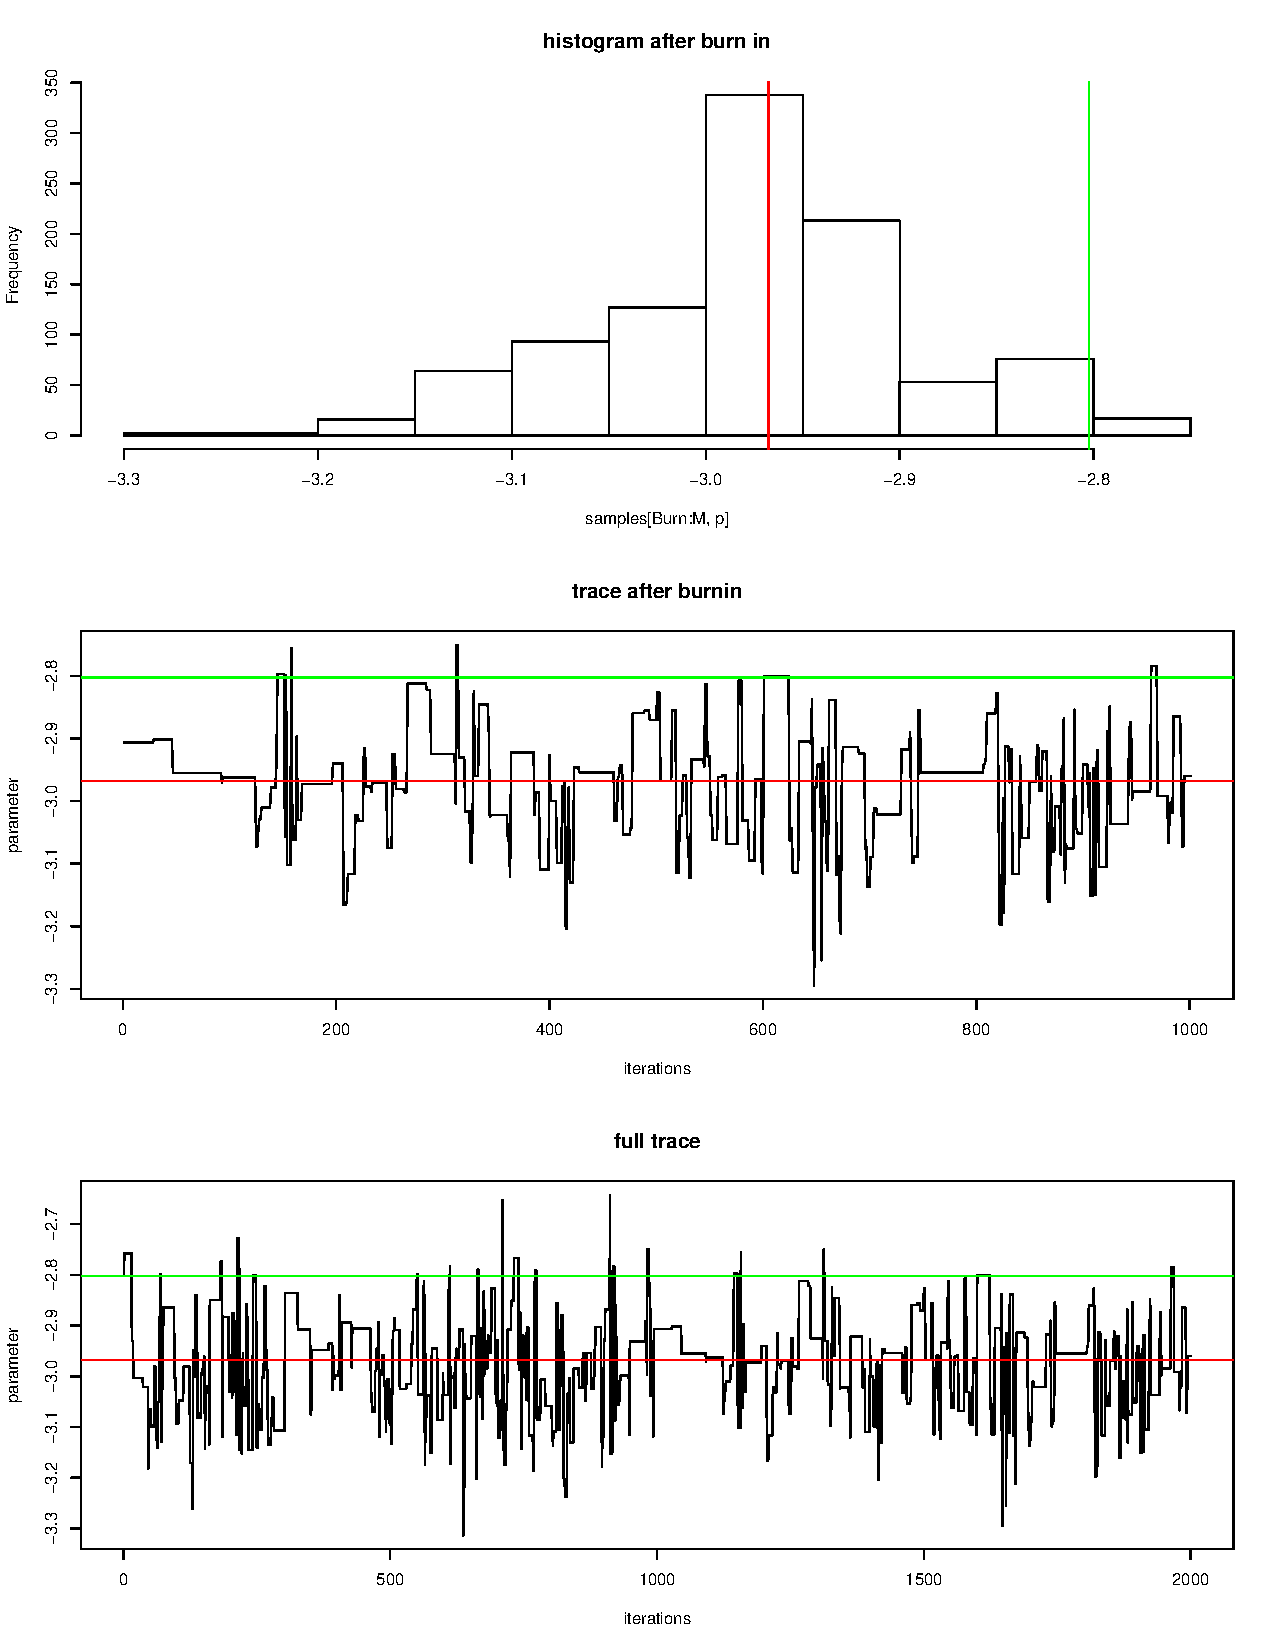
\includegraphics[scale=0.4]{1}  % scales figure to 35%\\
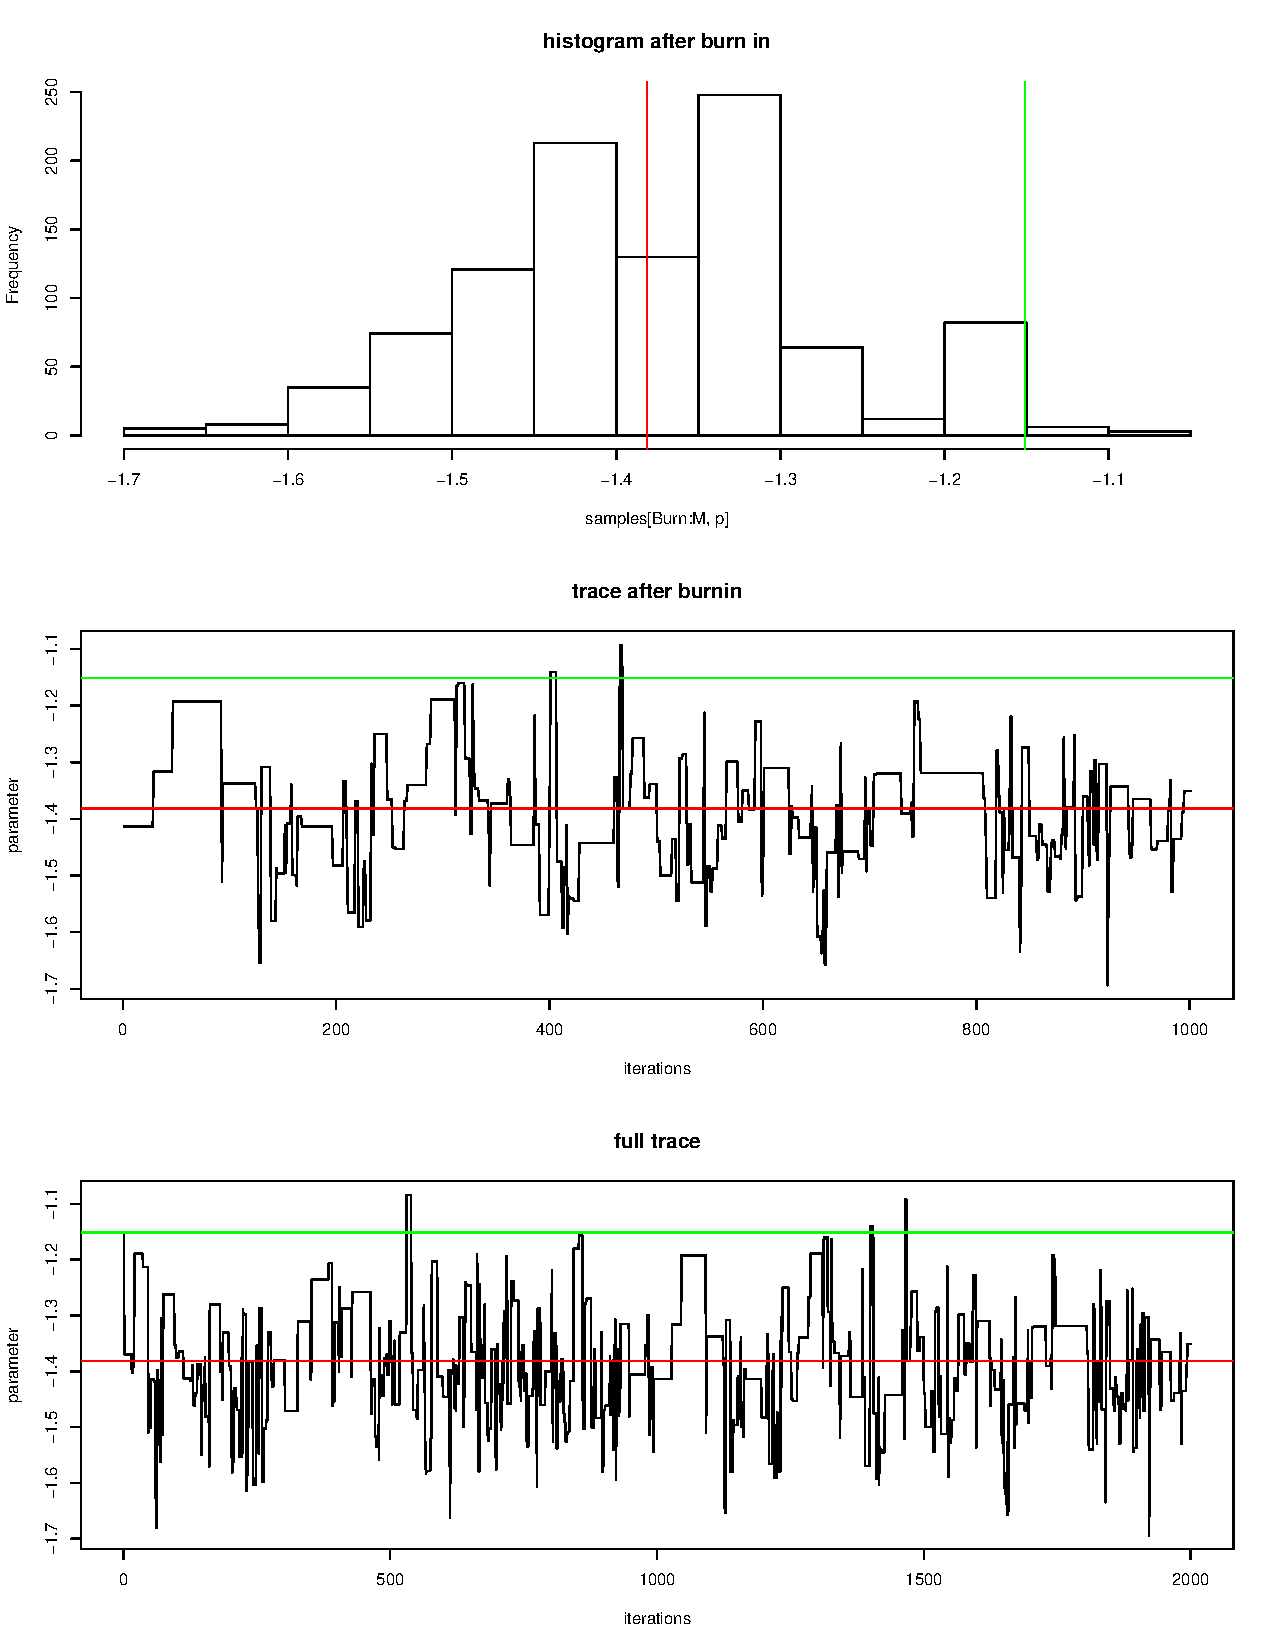
\includegraphics[scale=0.4]{2}
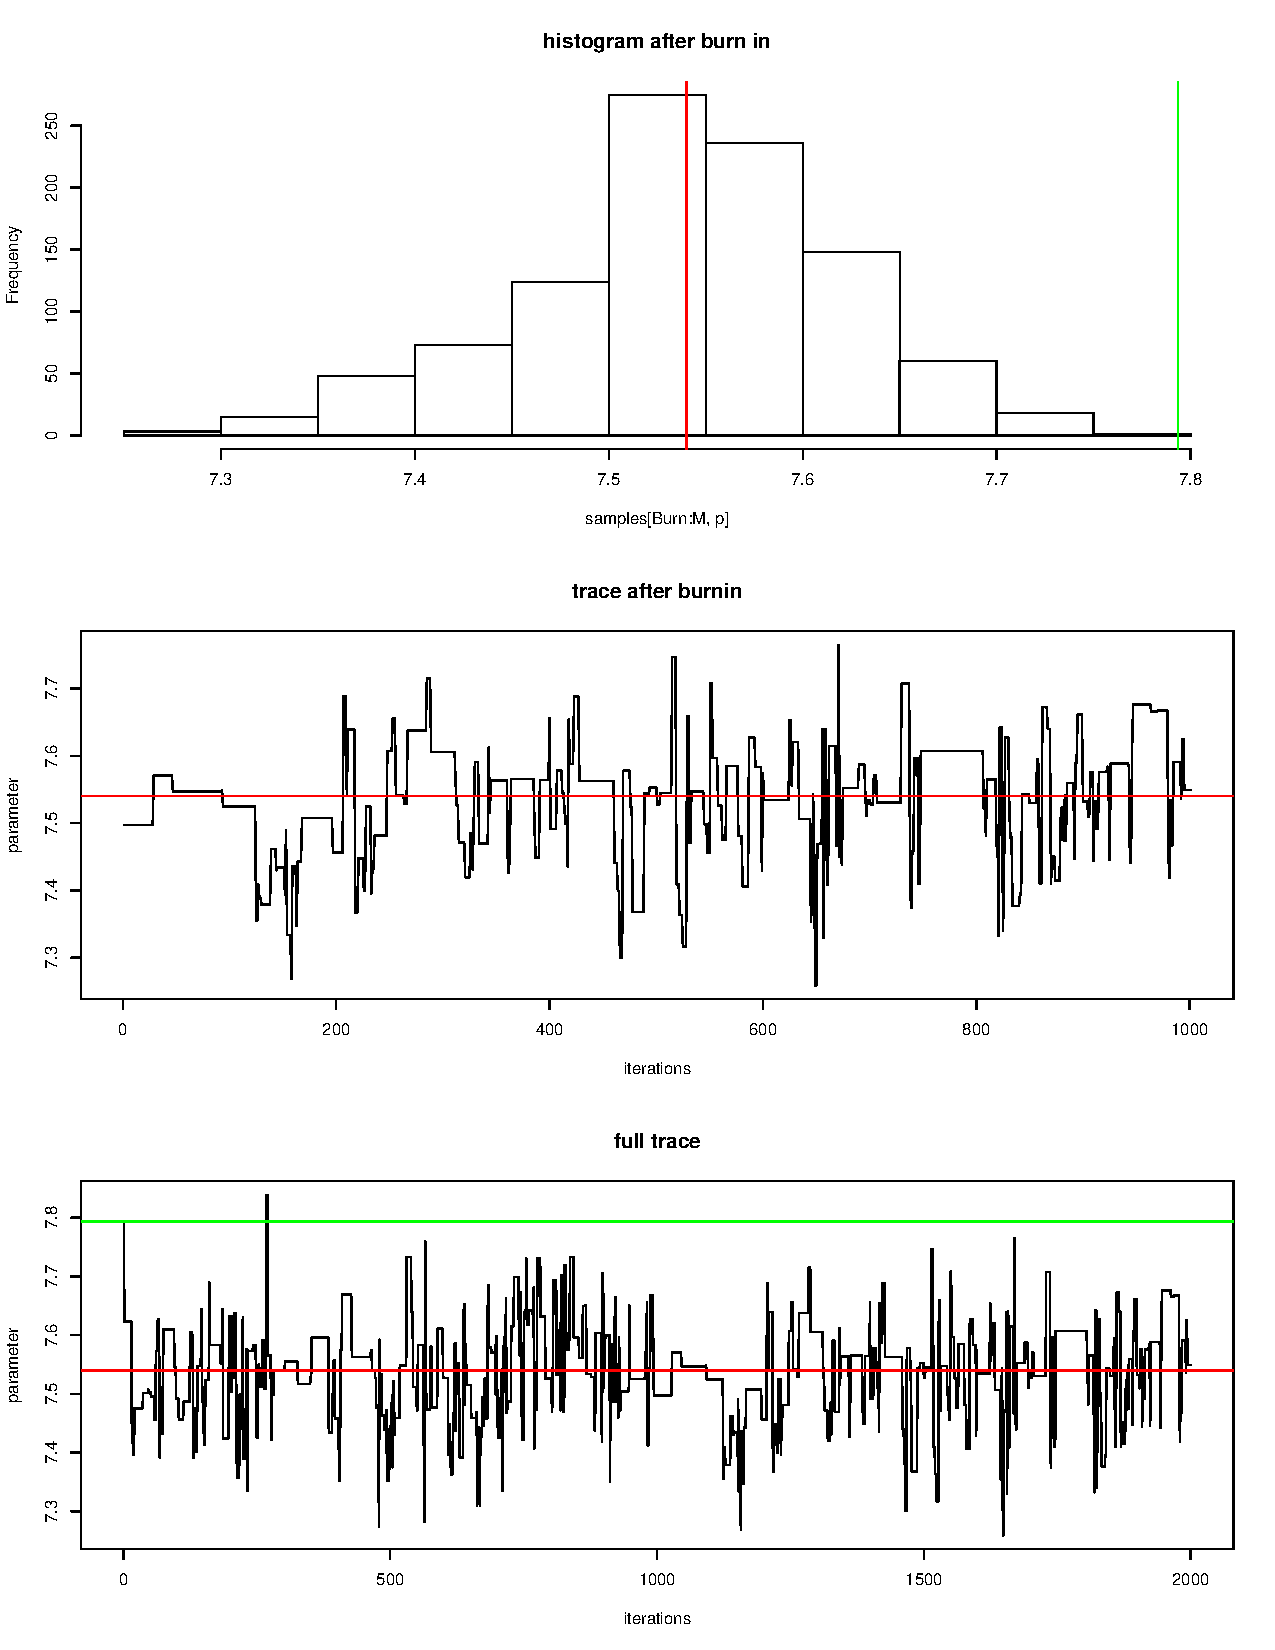
\includegraphics[scale=0.4]{3}
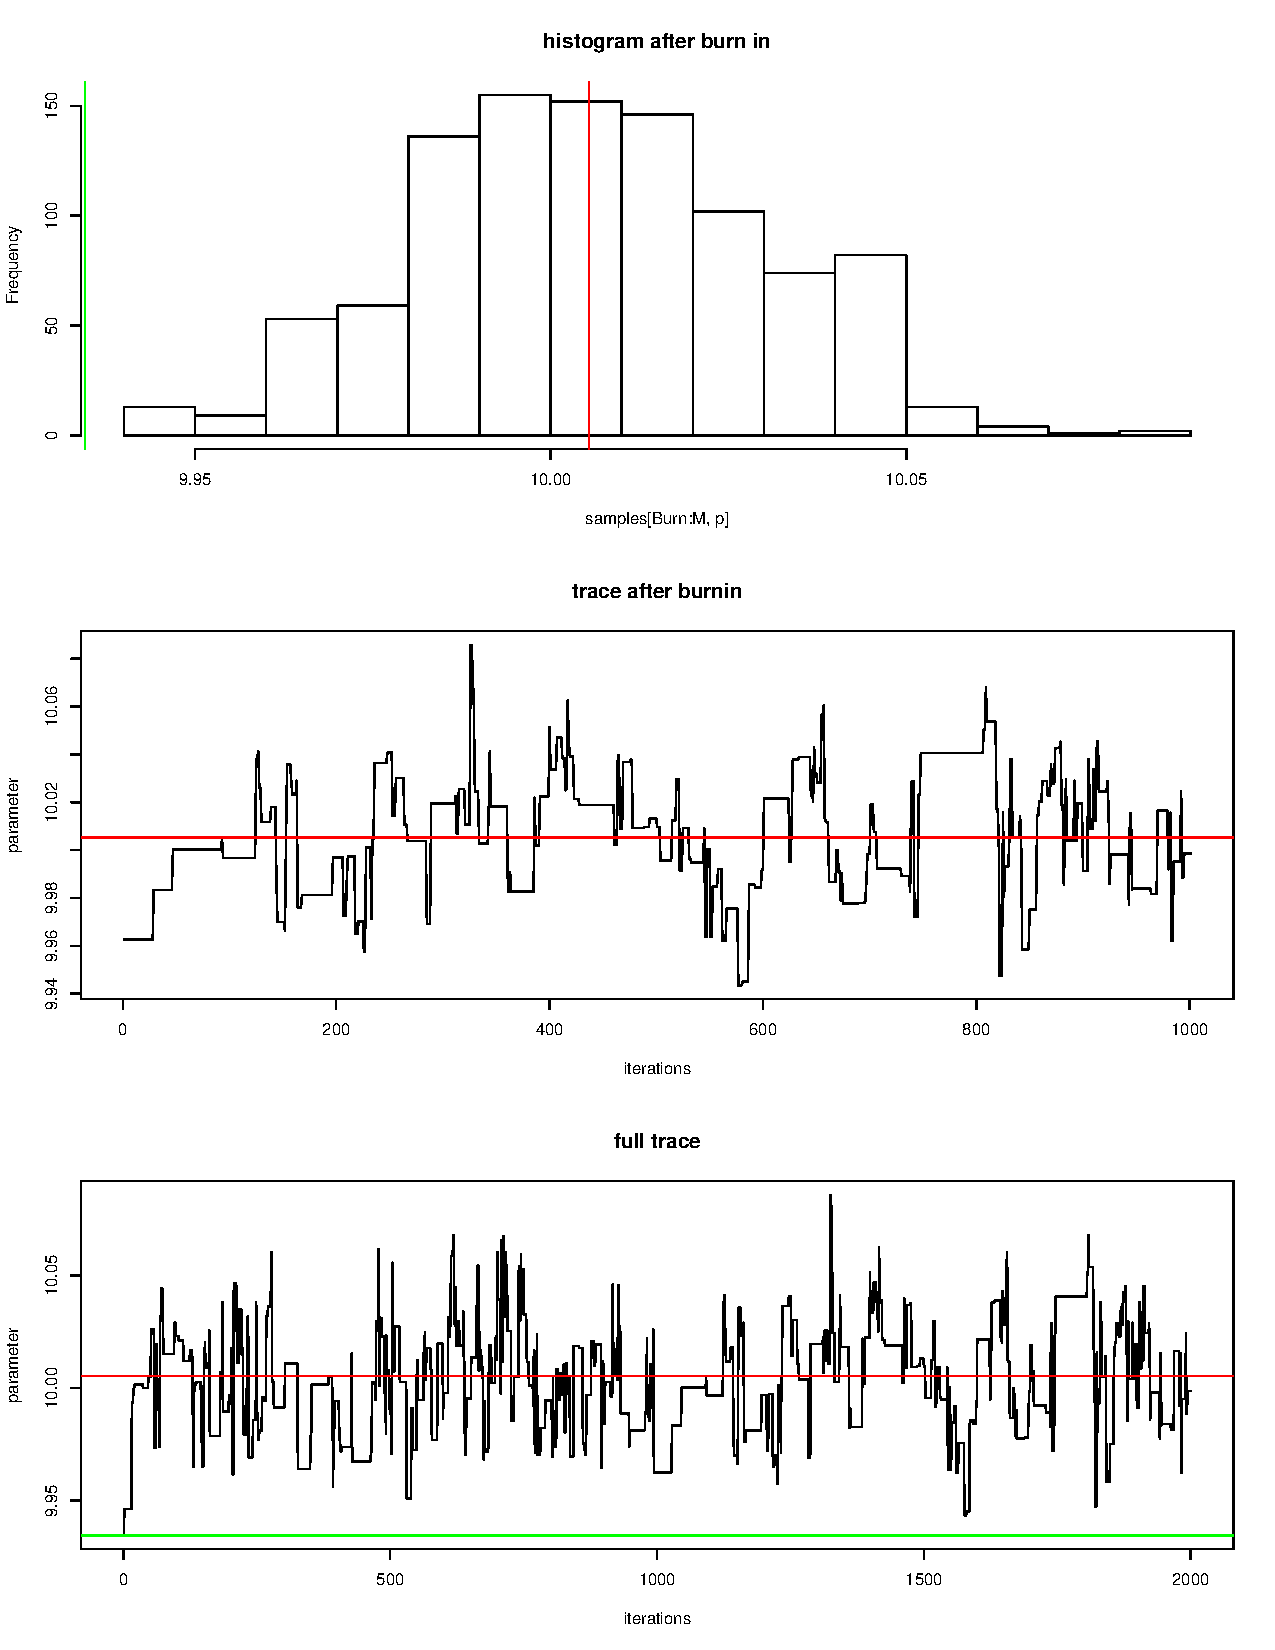
\includegraphics[scale=0.4]{4}
\clearpage
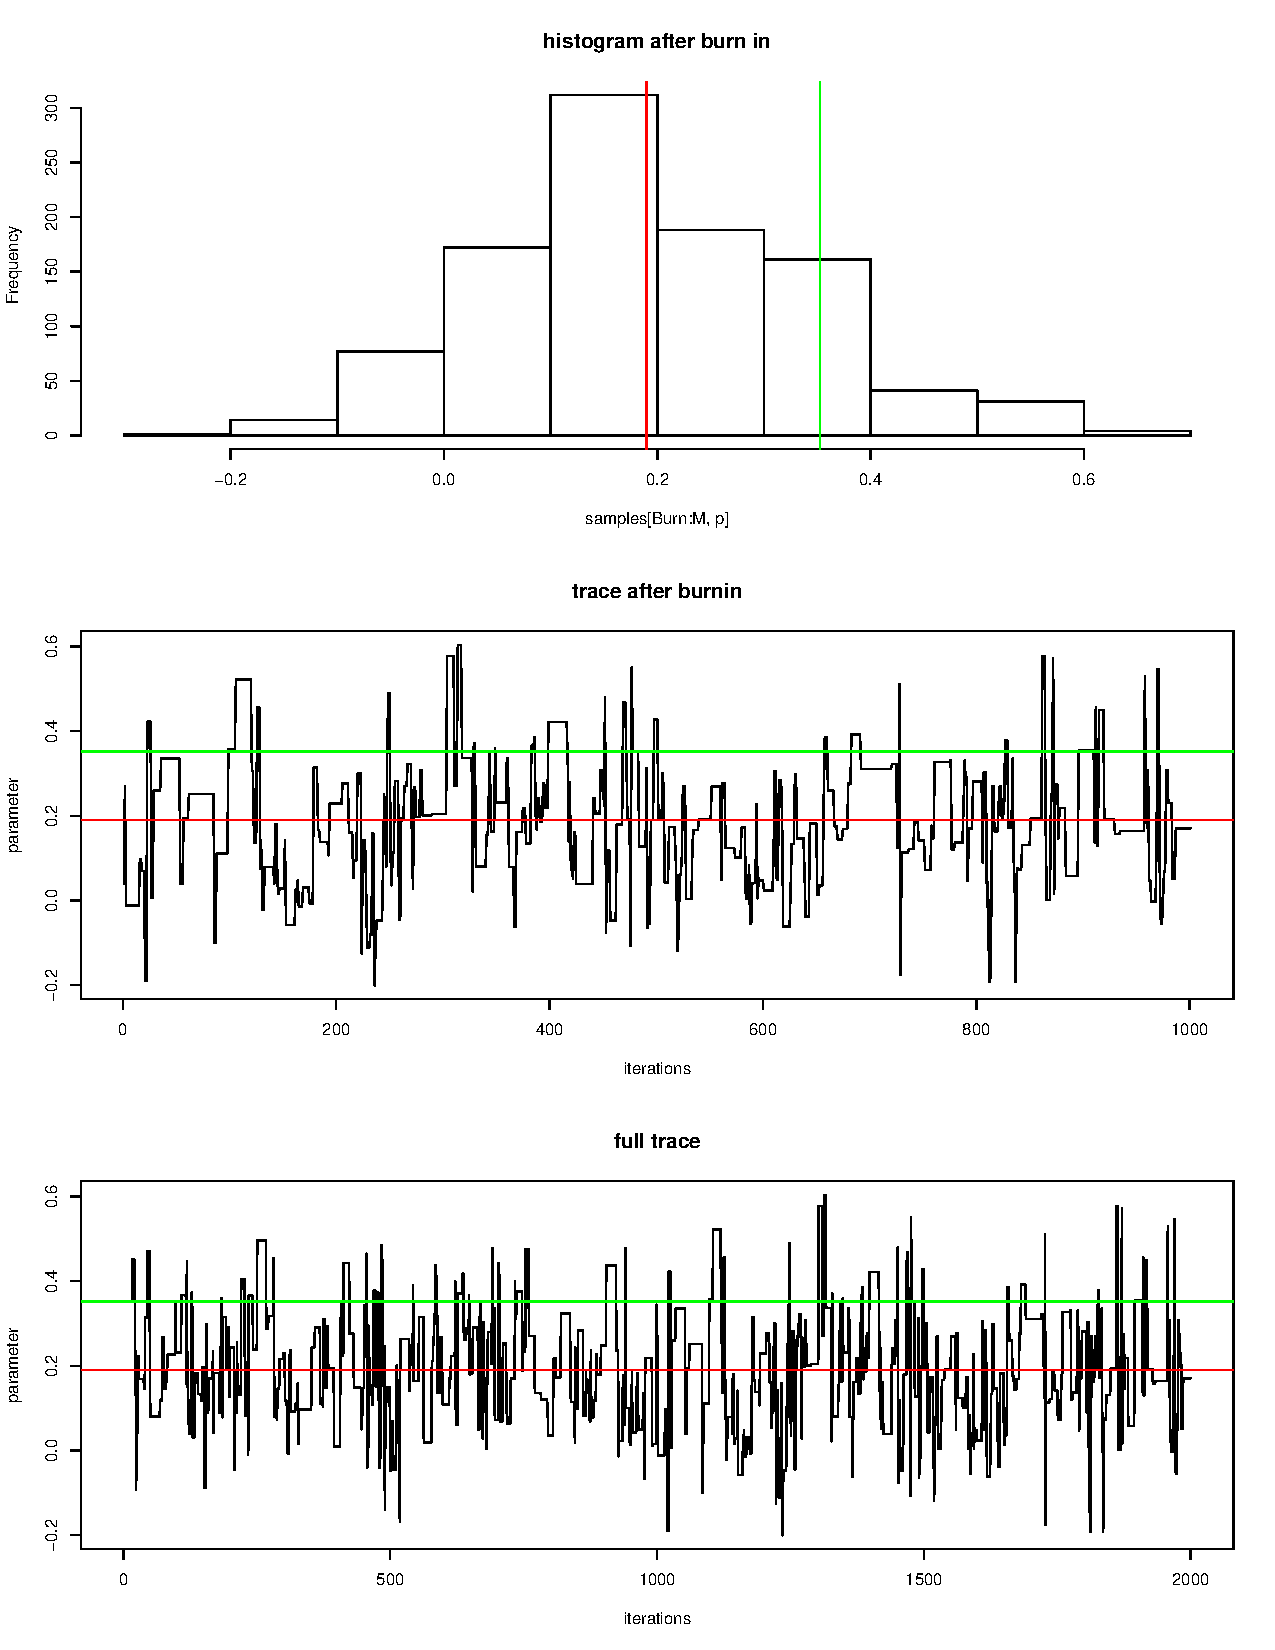
\includegraphics[scale=0.4]{5}  % scales figure to 35%\\
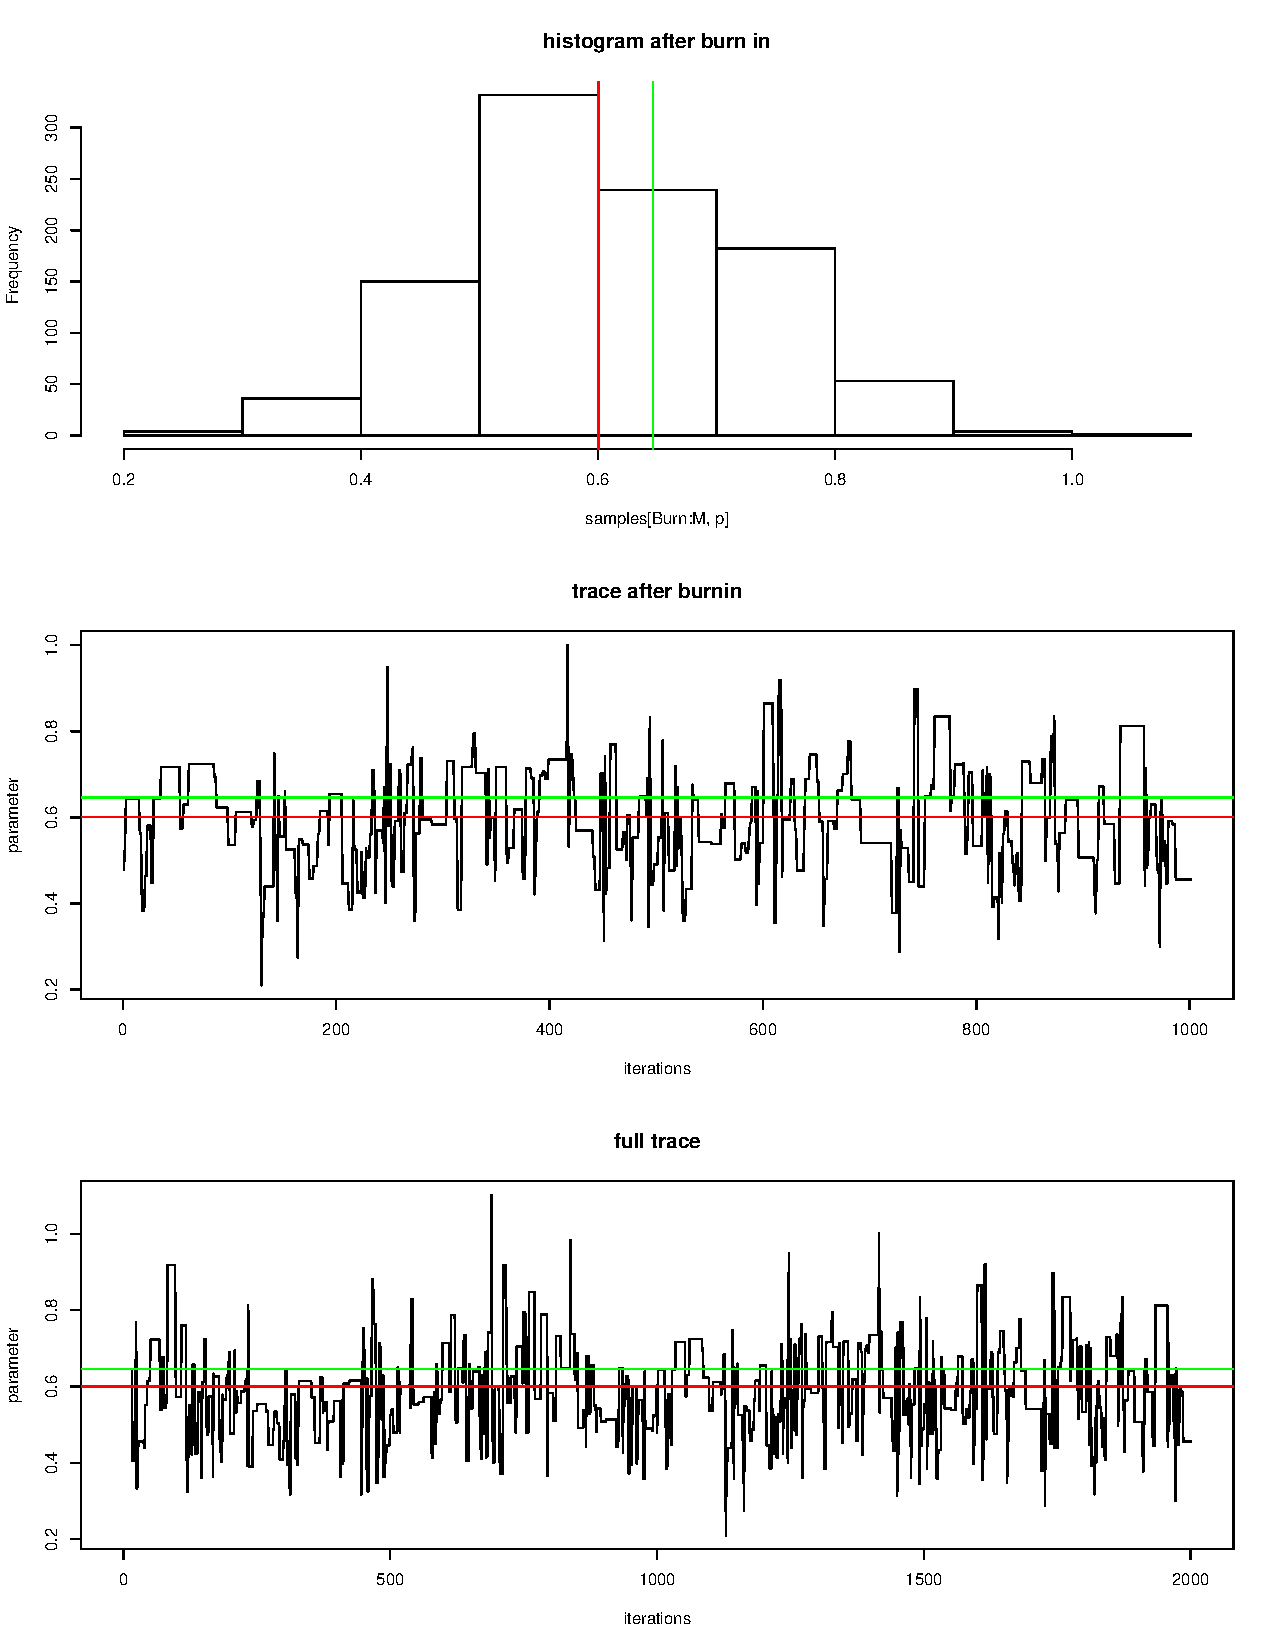
\includegraphics[scale=0.4]{6}
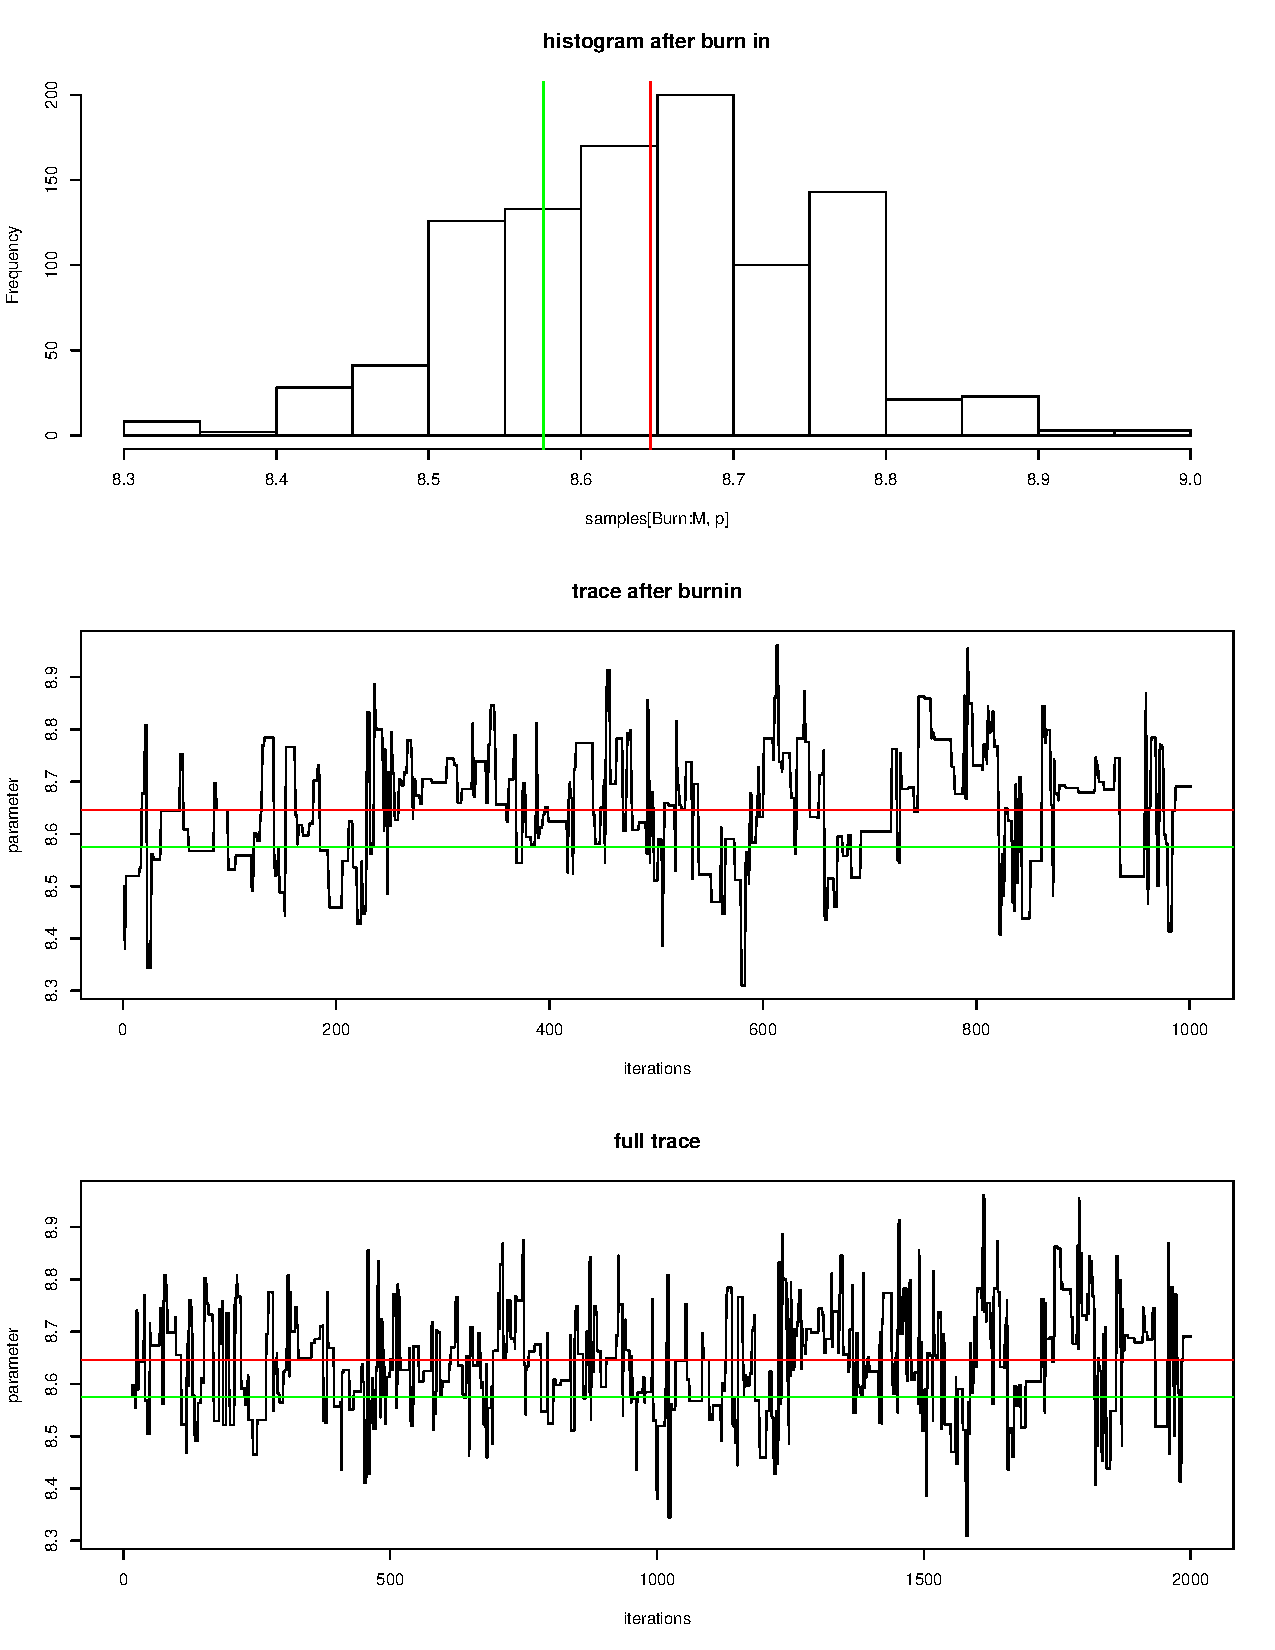
\includegraphics[scale=0.4]{7}
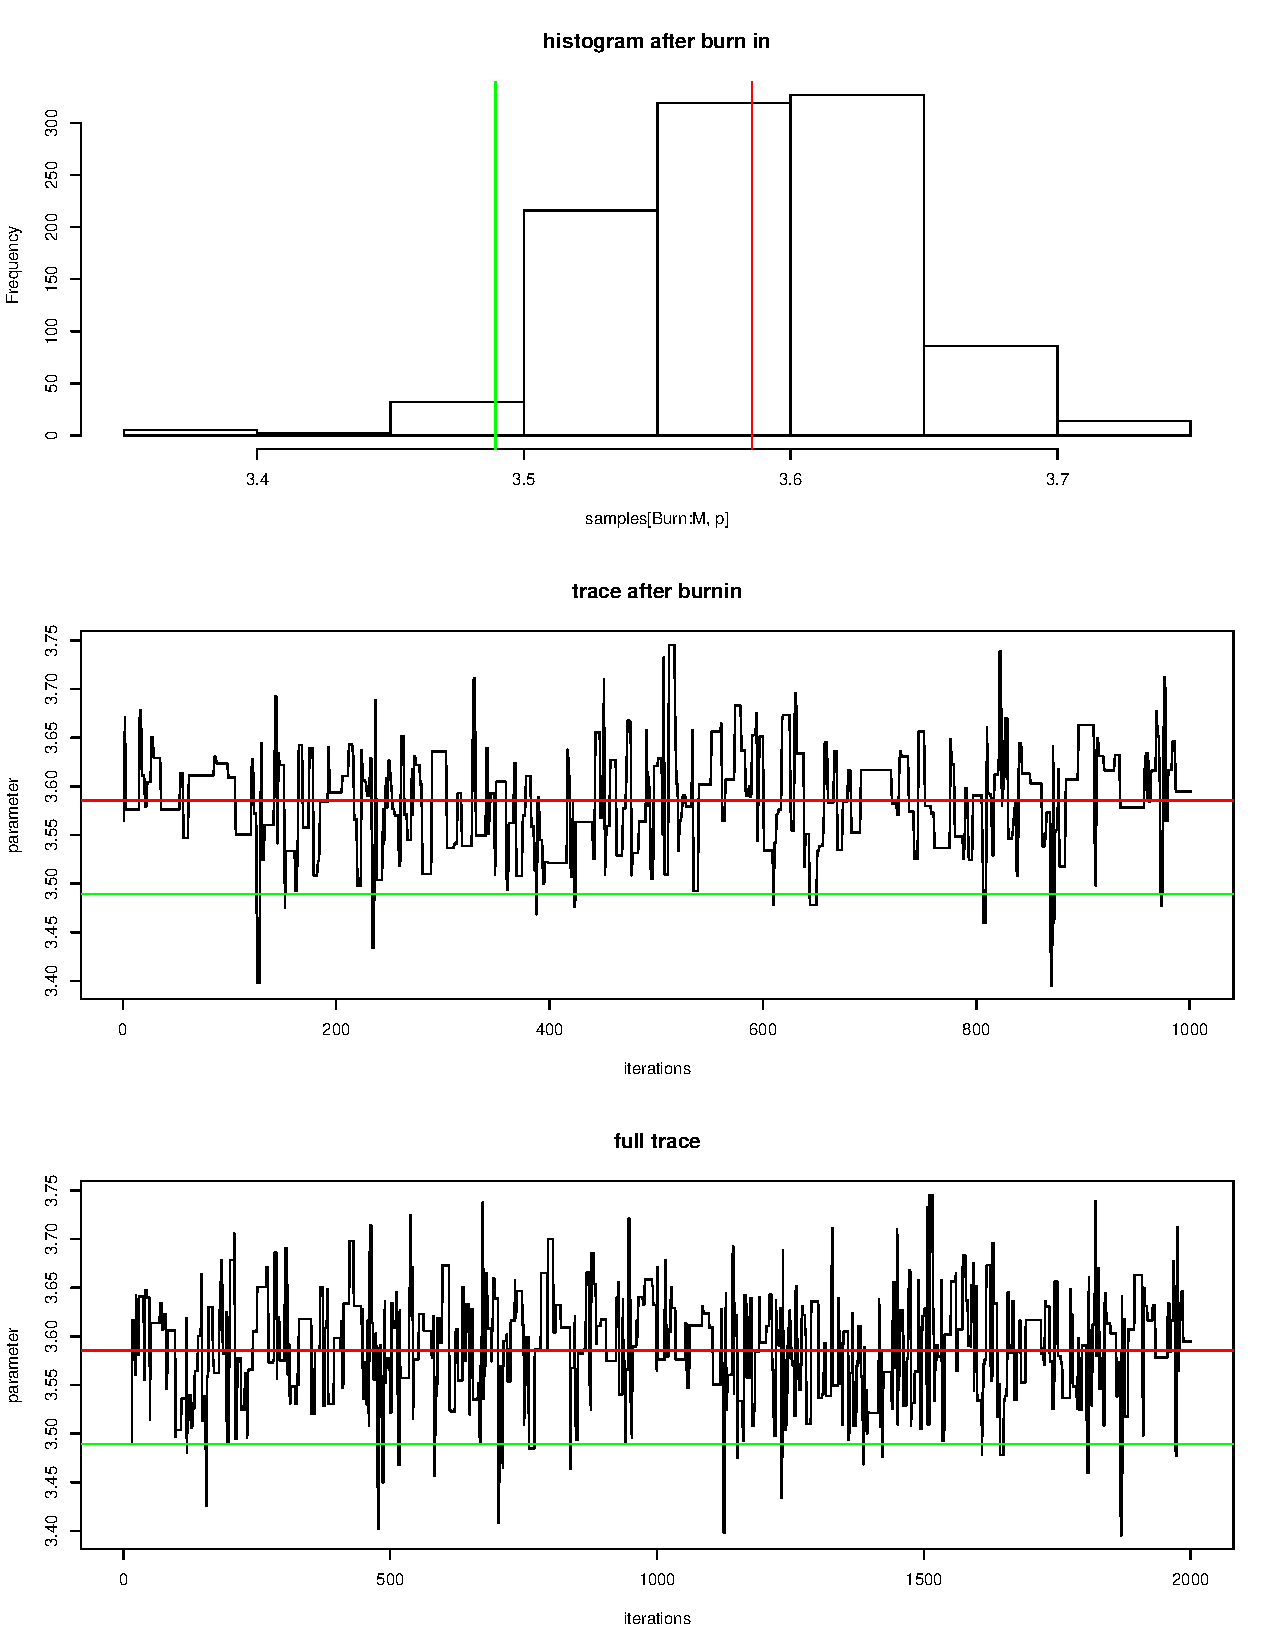
\includegraphics[scale=0.4]{8}
\clearpage
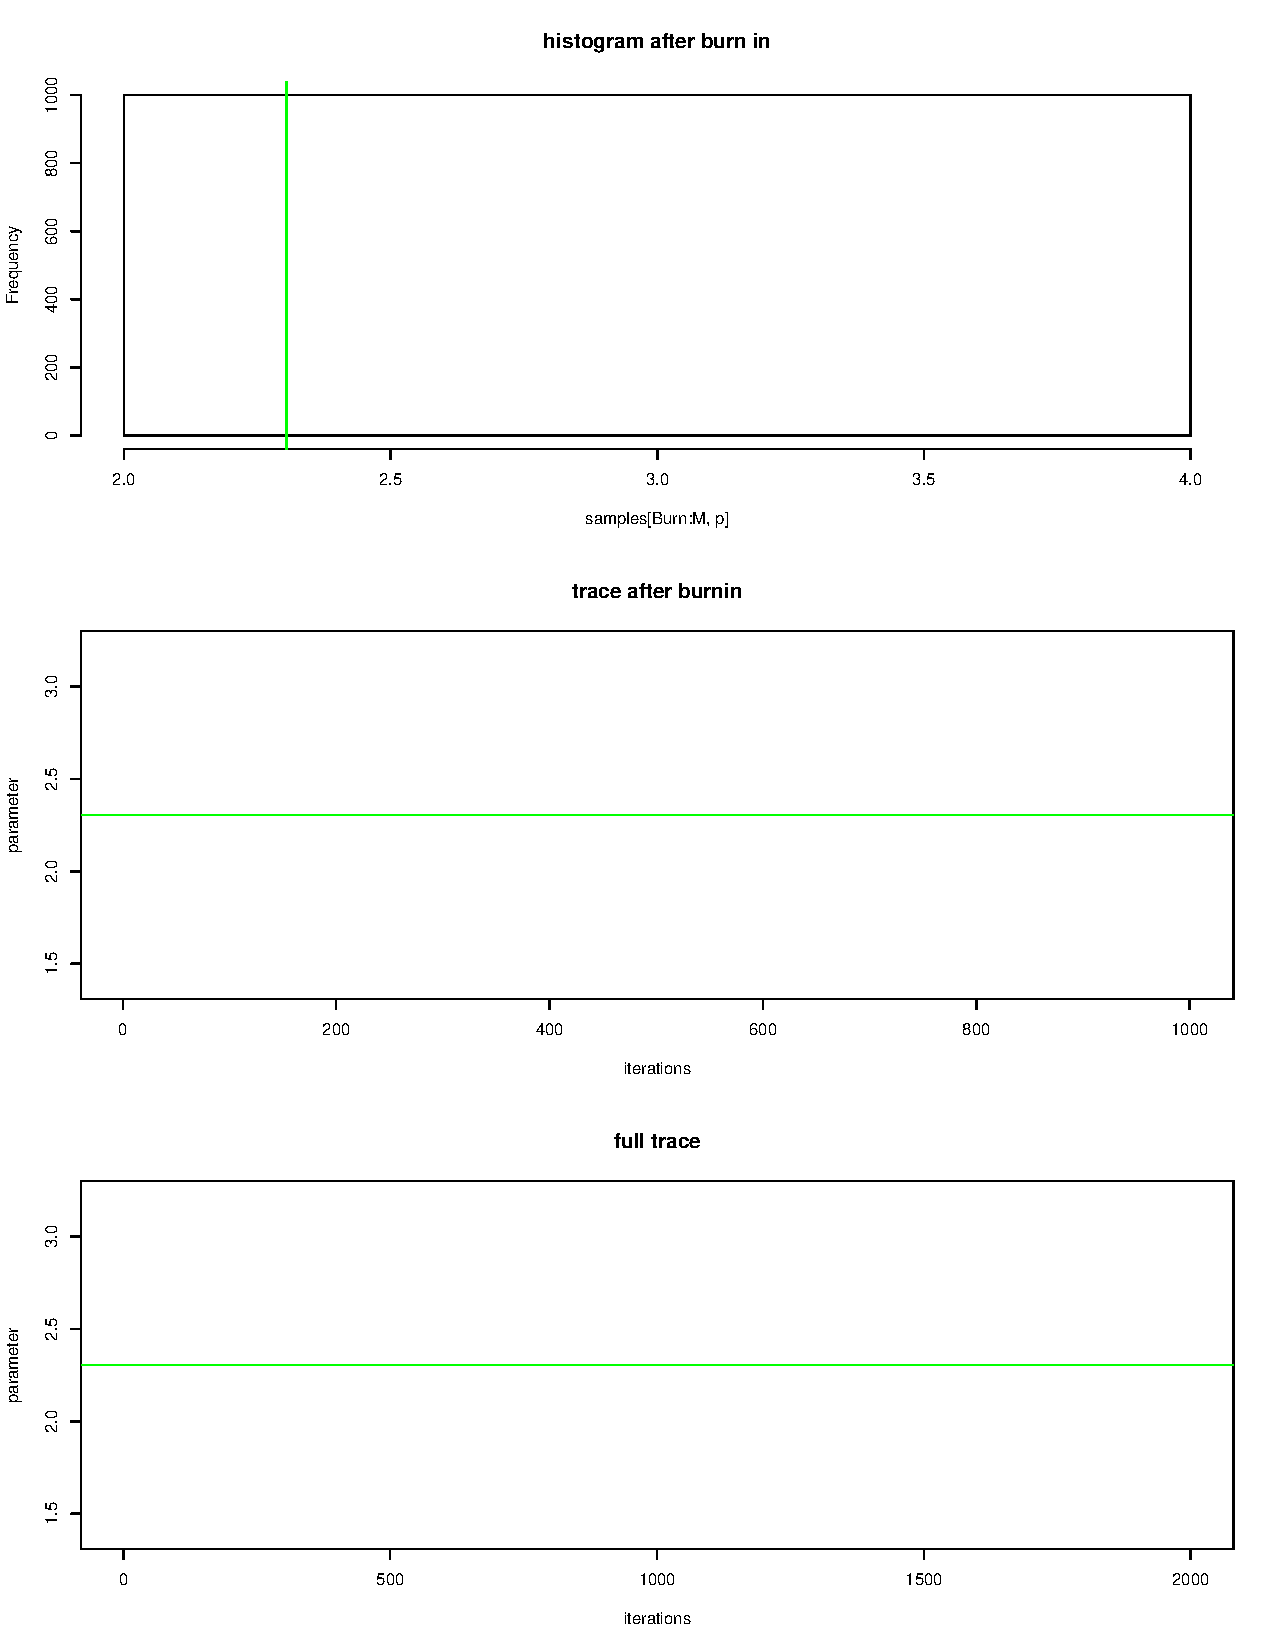
\includegraphics[scale=0.4]{9}  % scales figure to 35%\\
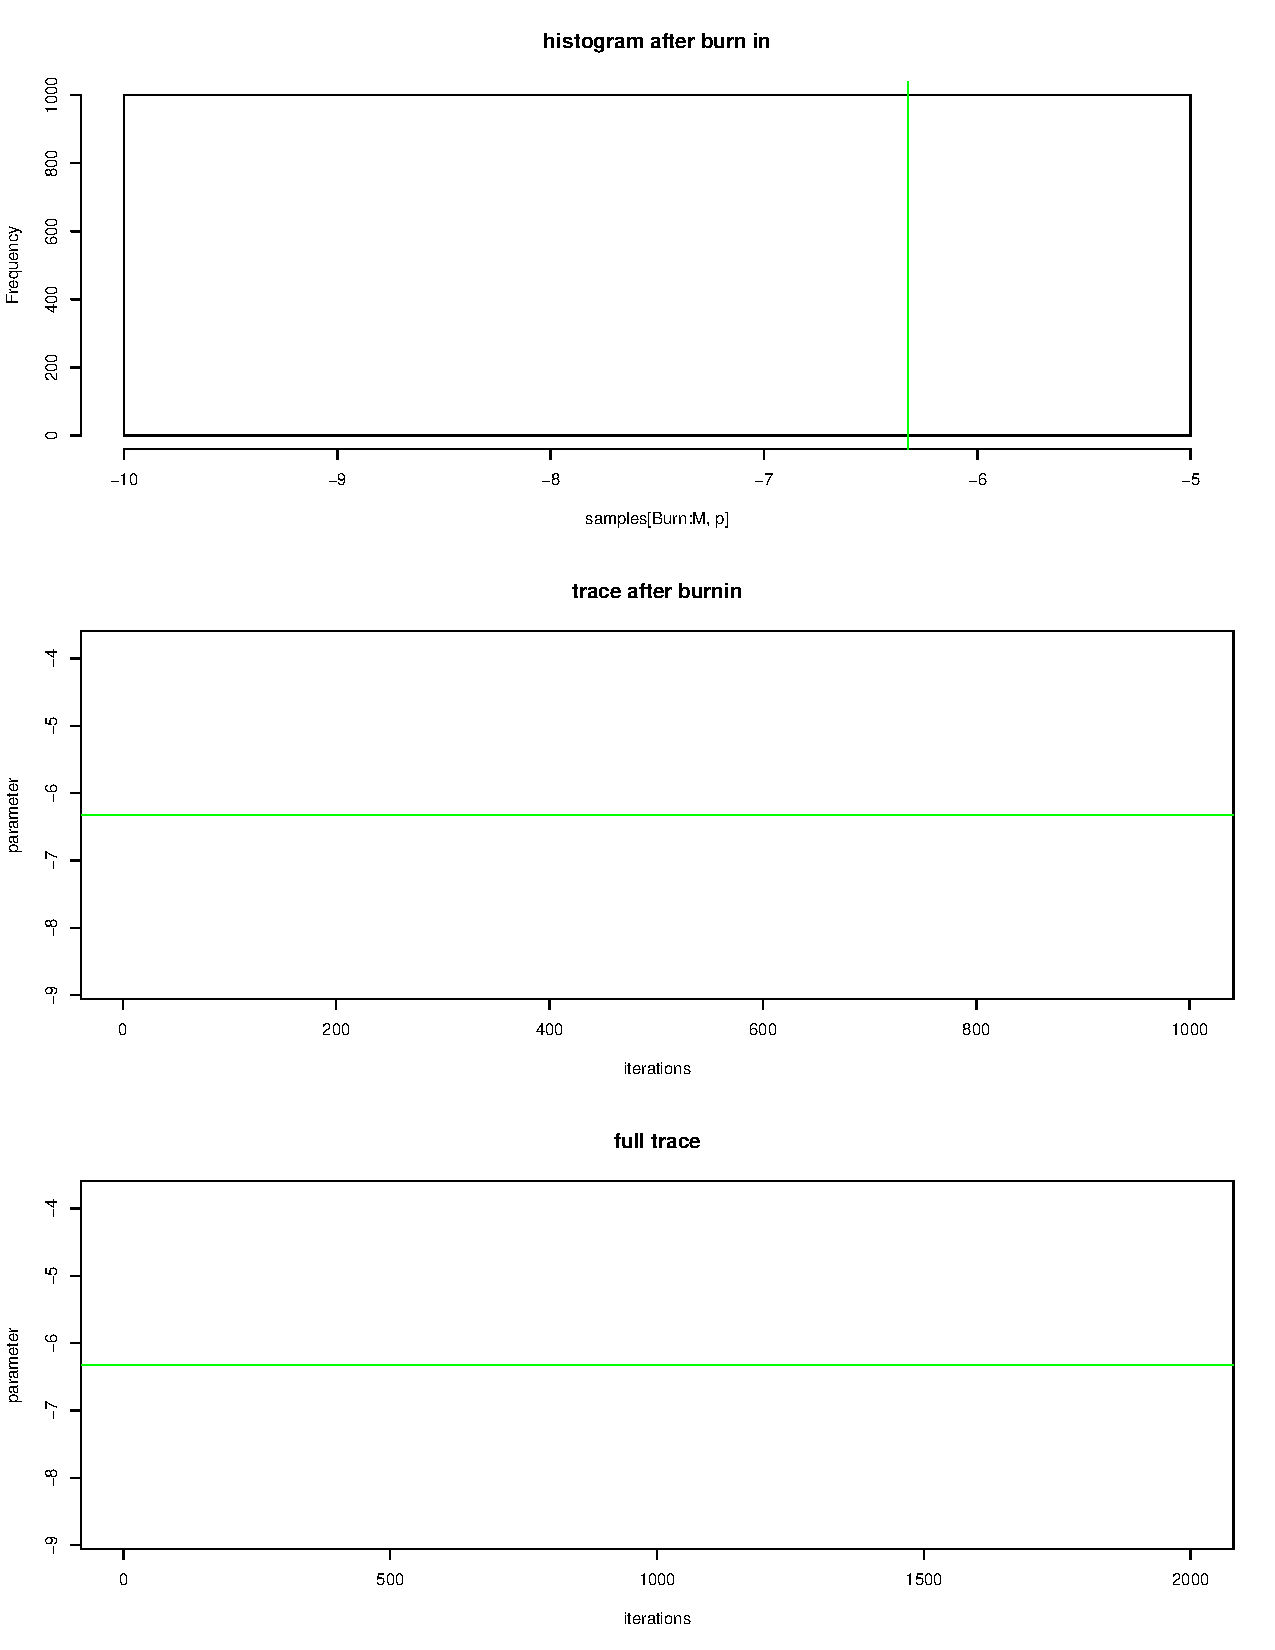
\includegraphics[scale=0.4]{10}
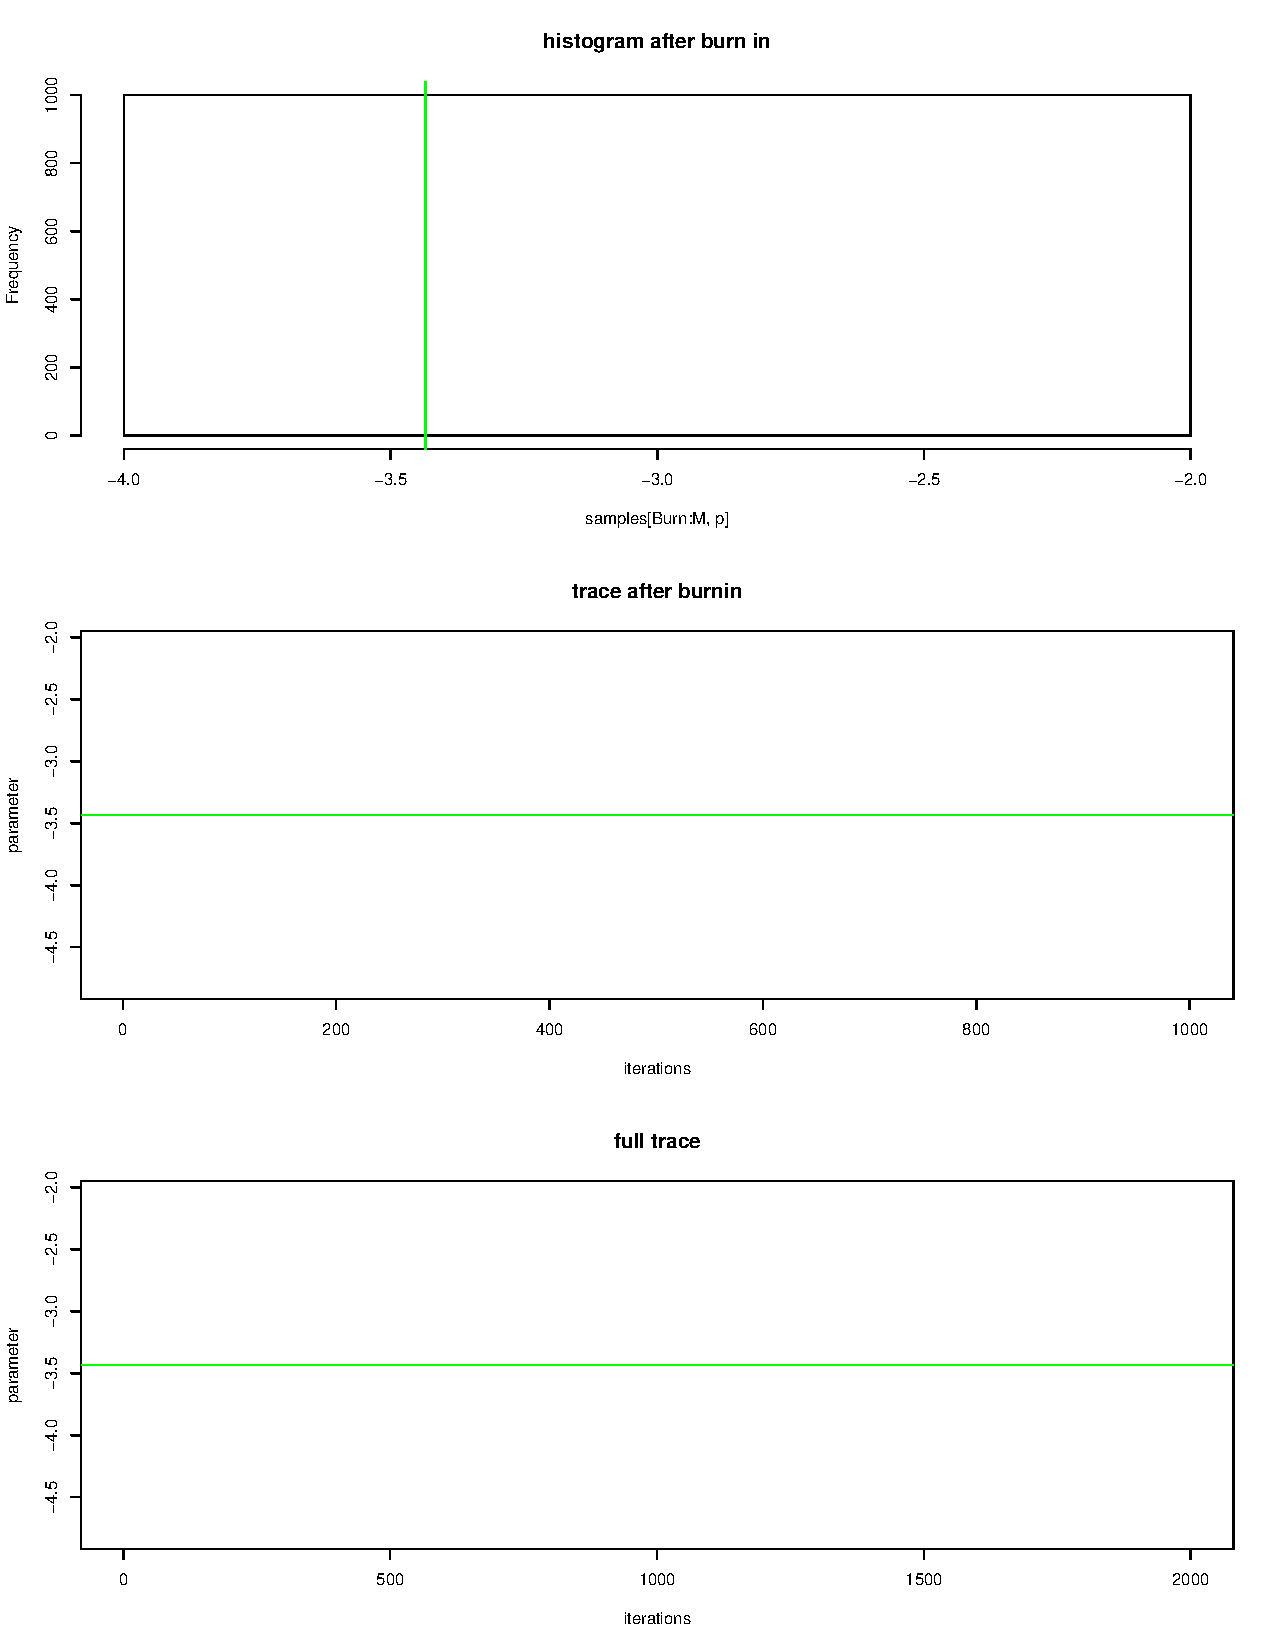
\includegraphics[scale=0.4]{11}
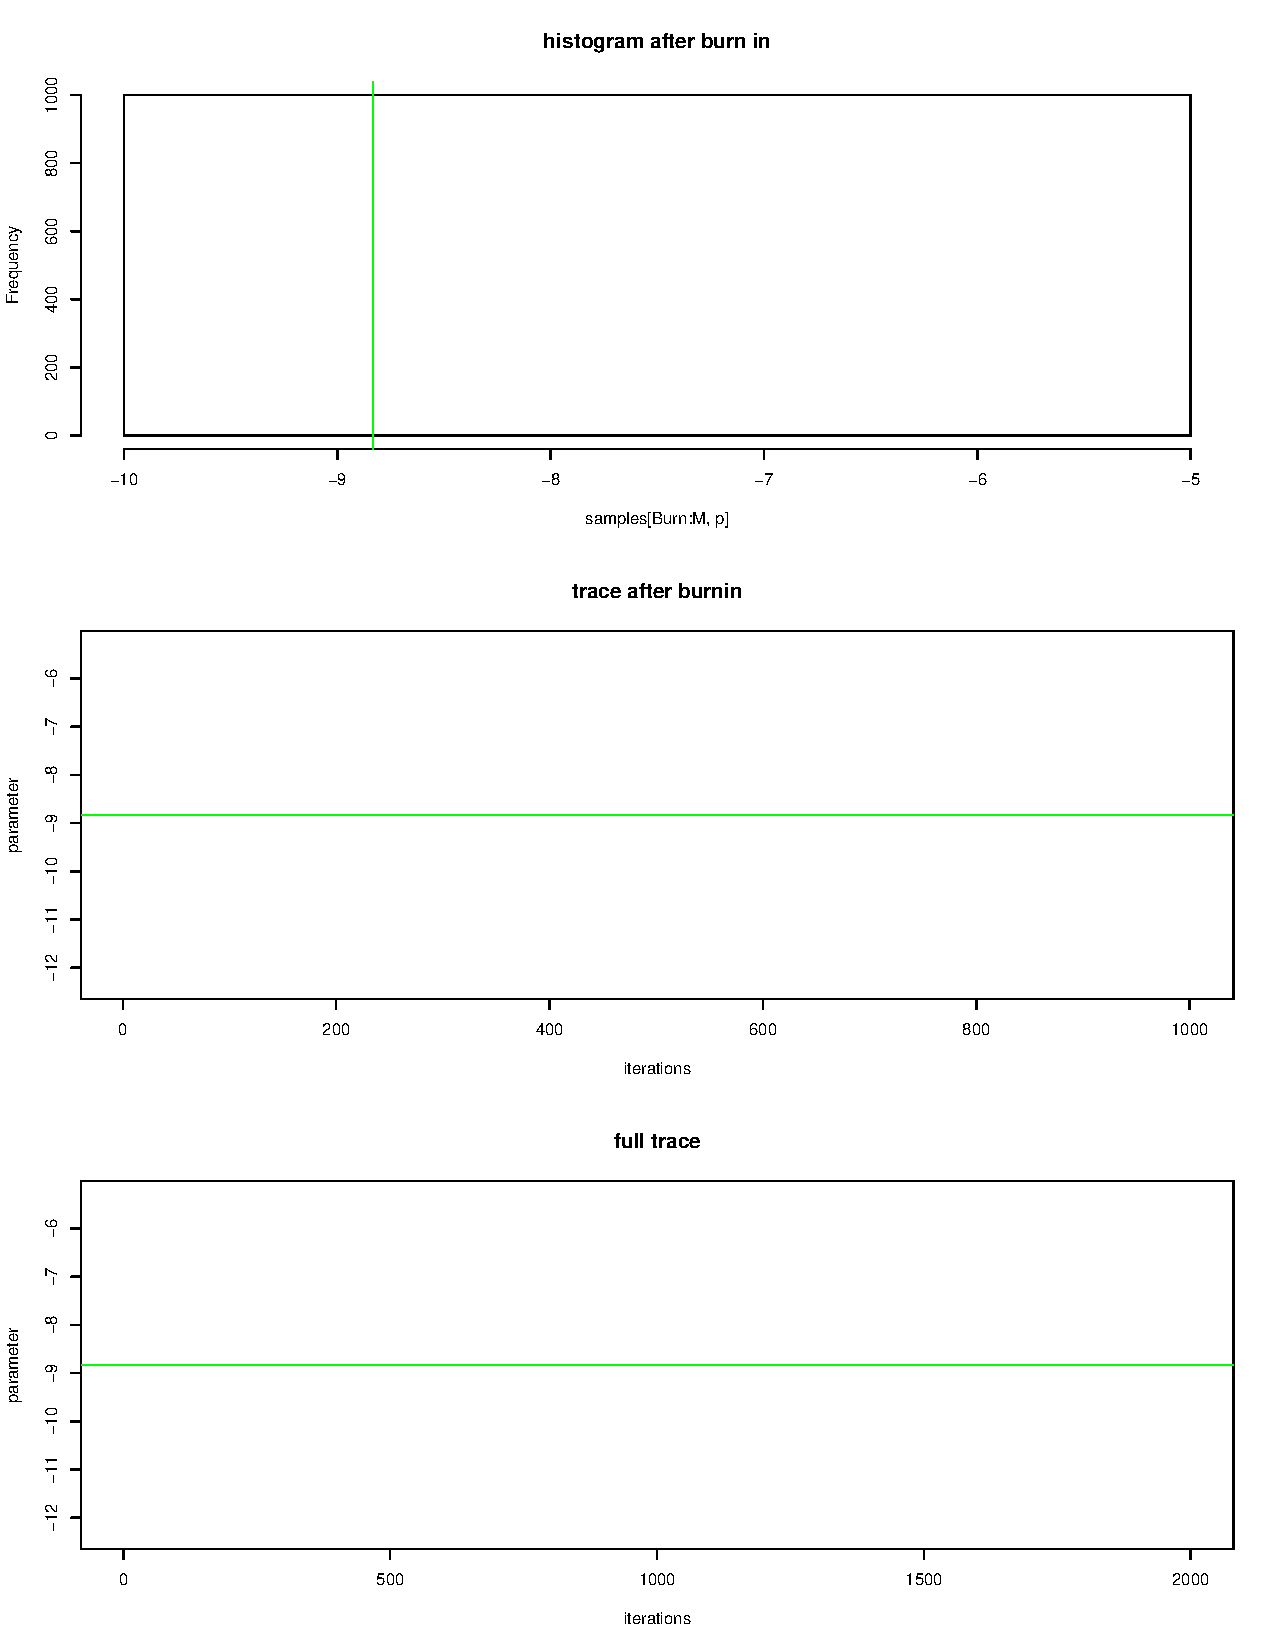
\includegraphics[scale=0.4]{12}
\clearpage
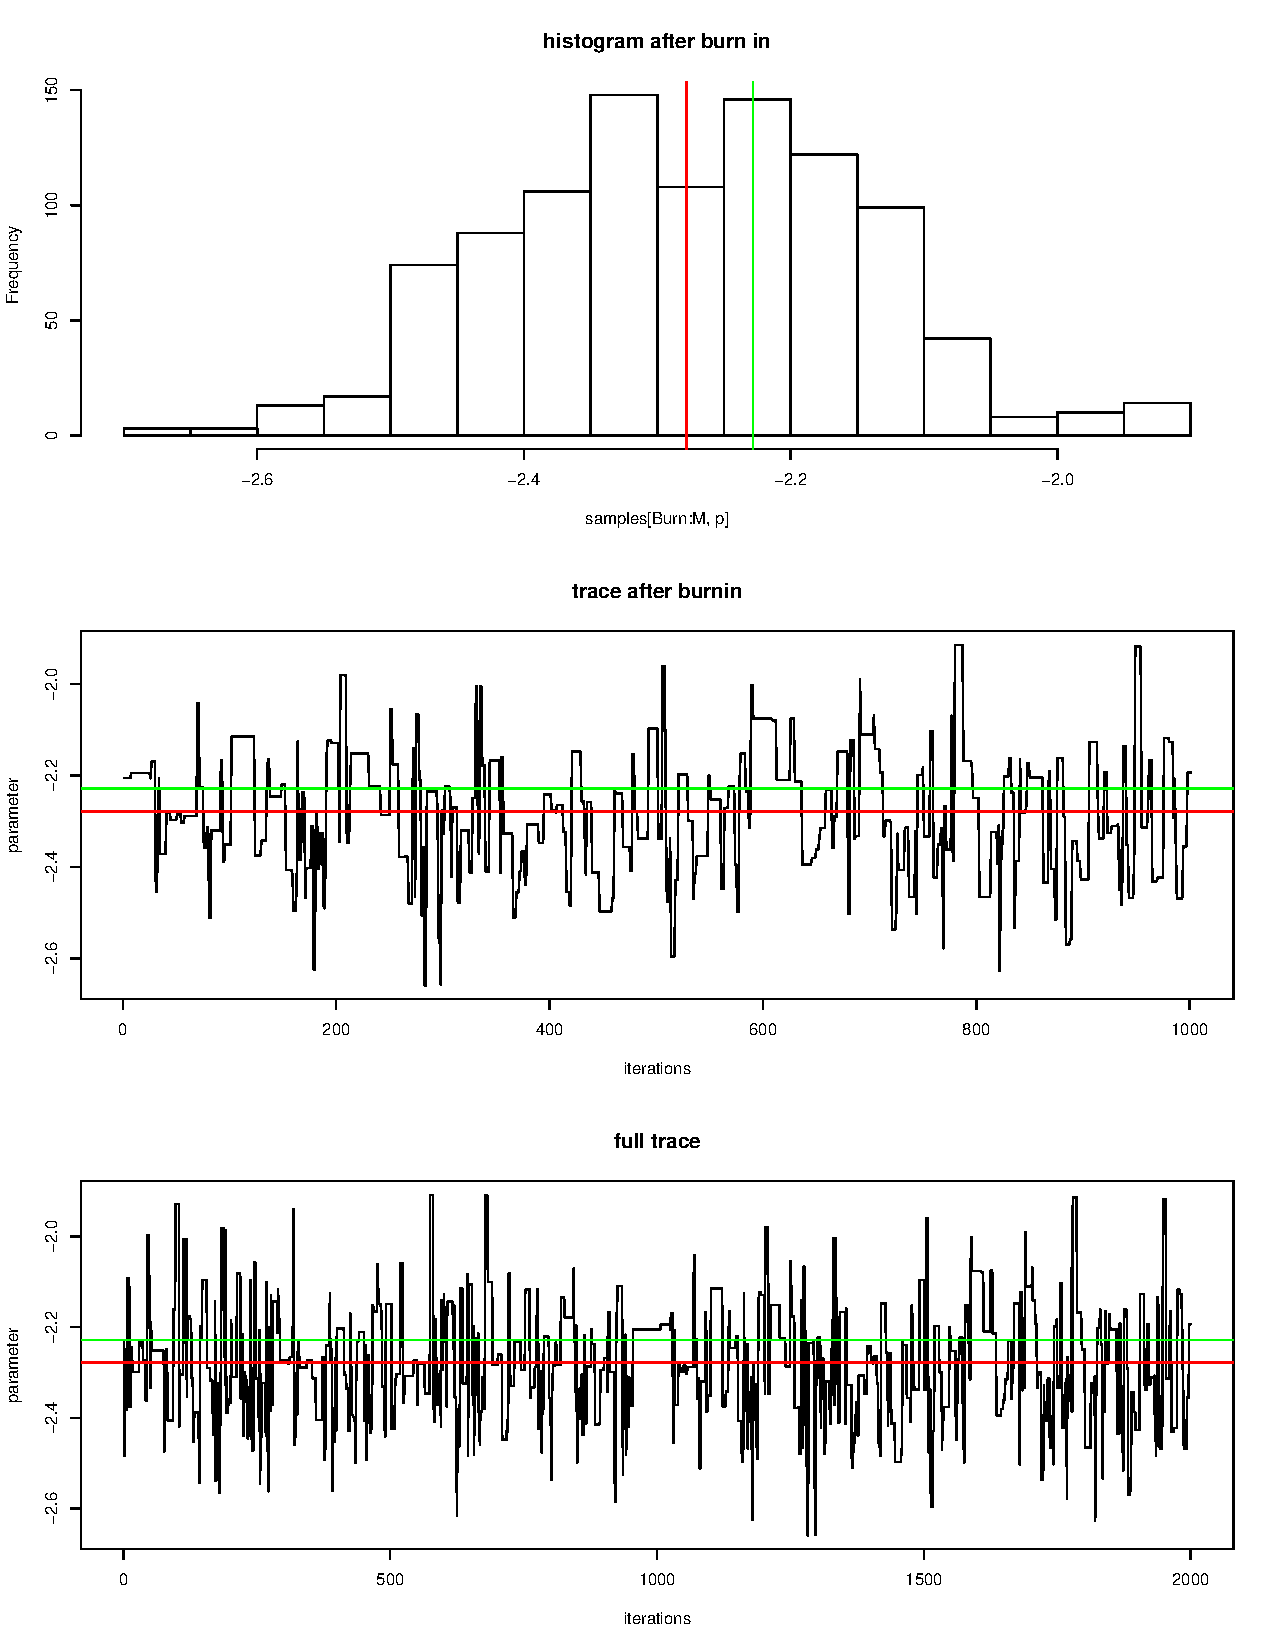
\includegraphics[scale=0.4]{13}  % scales figure to 35%\\
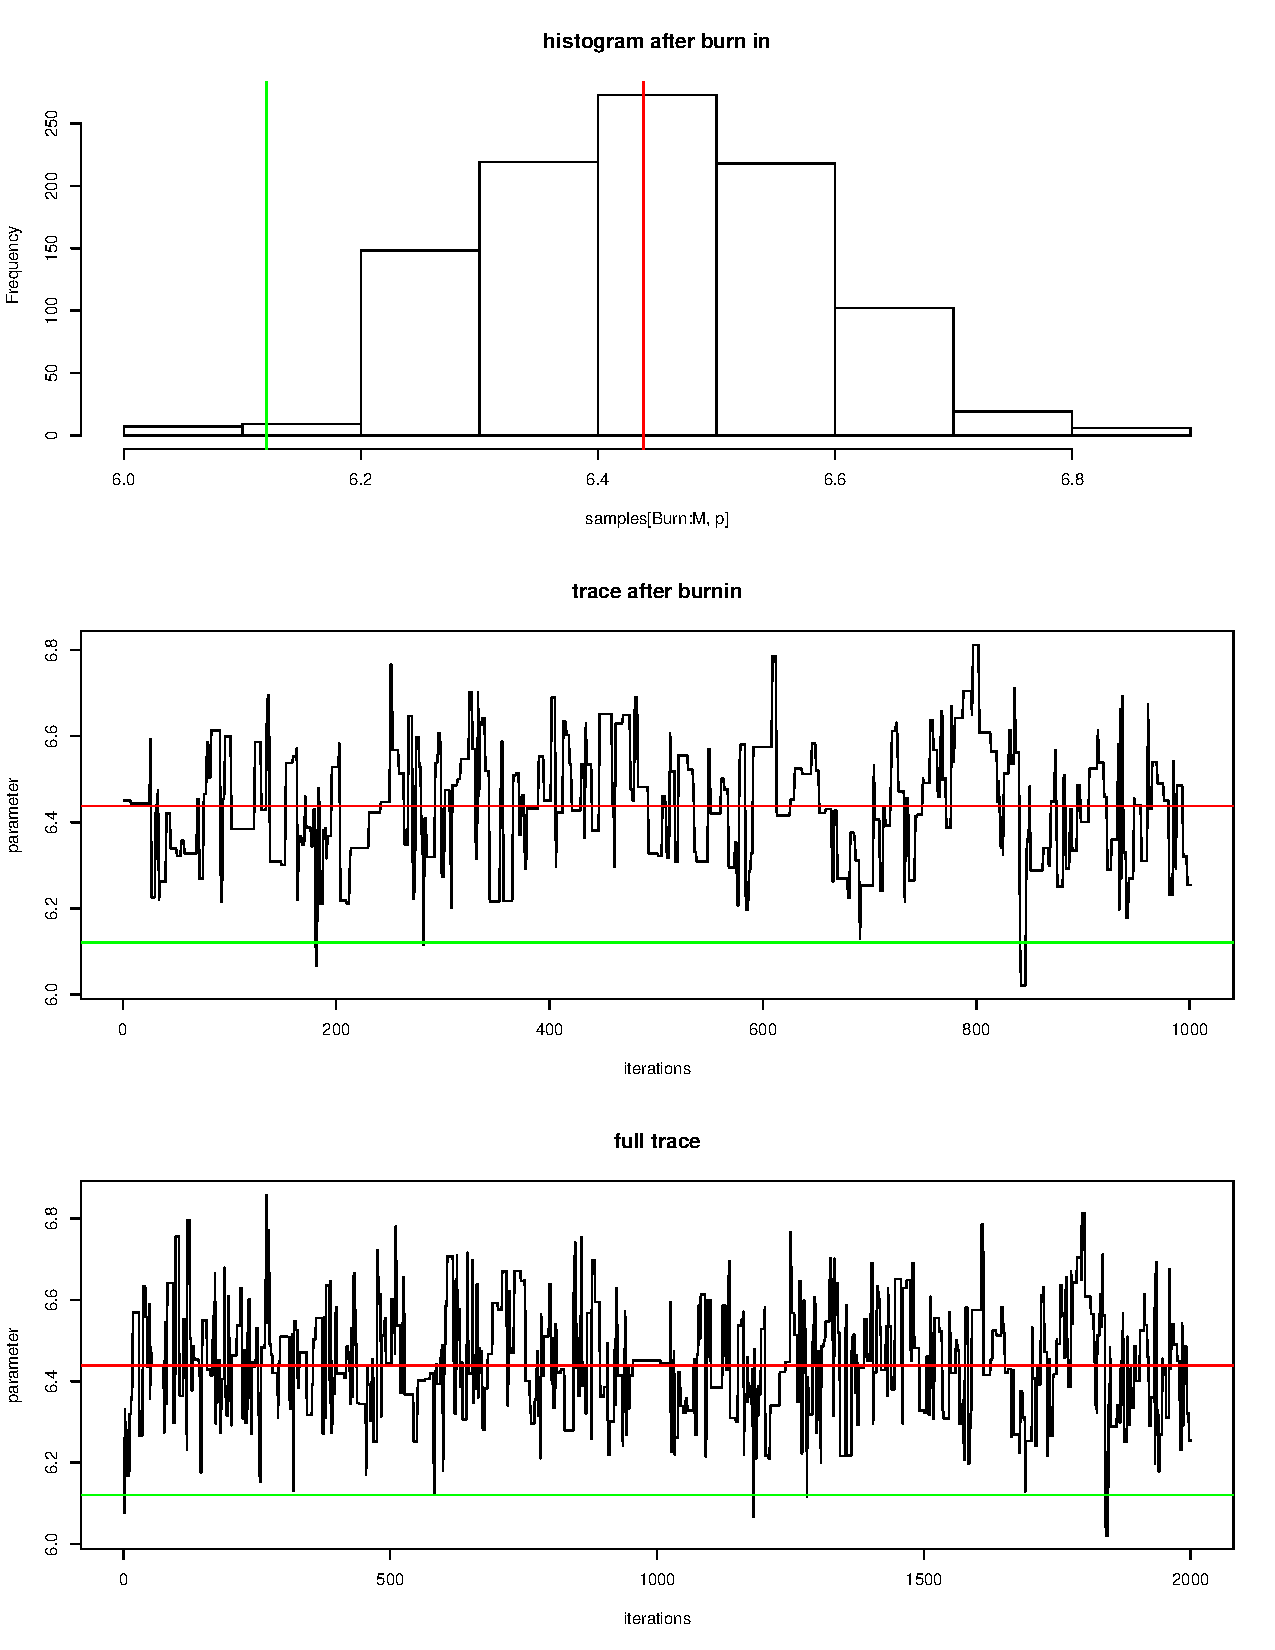
\includegraphics[scale=0.4]{14}
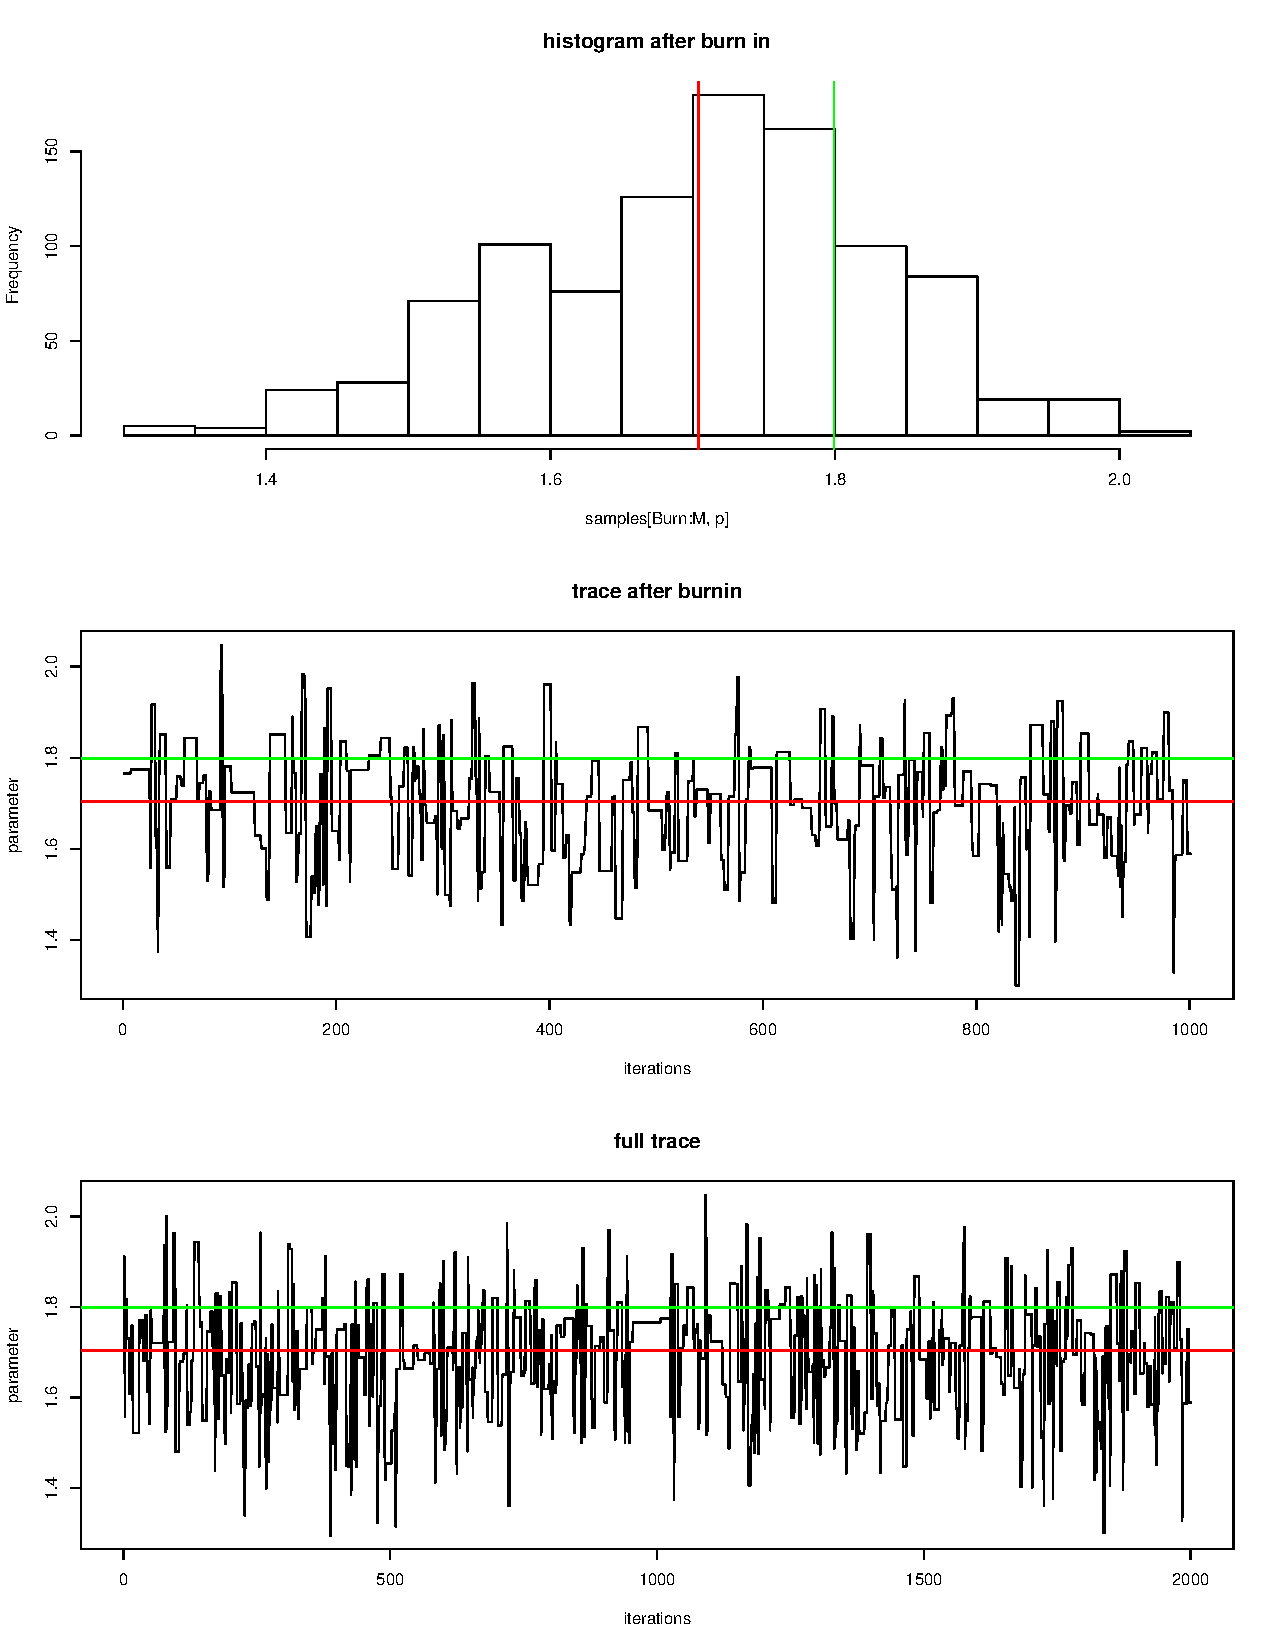
\includegraphics[scale=0.4]{15}
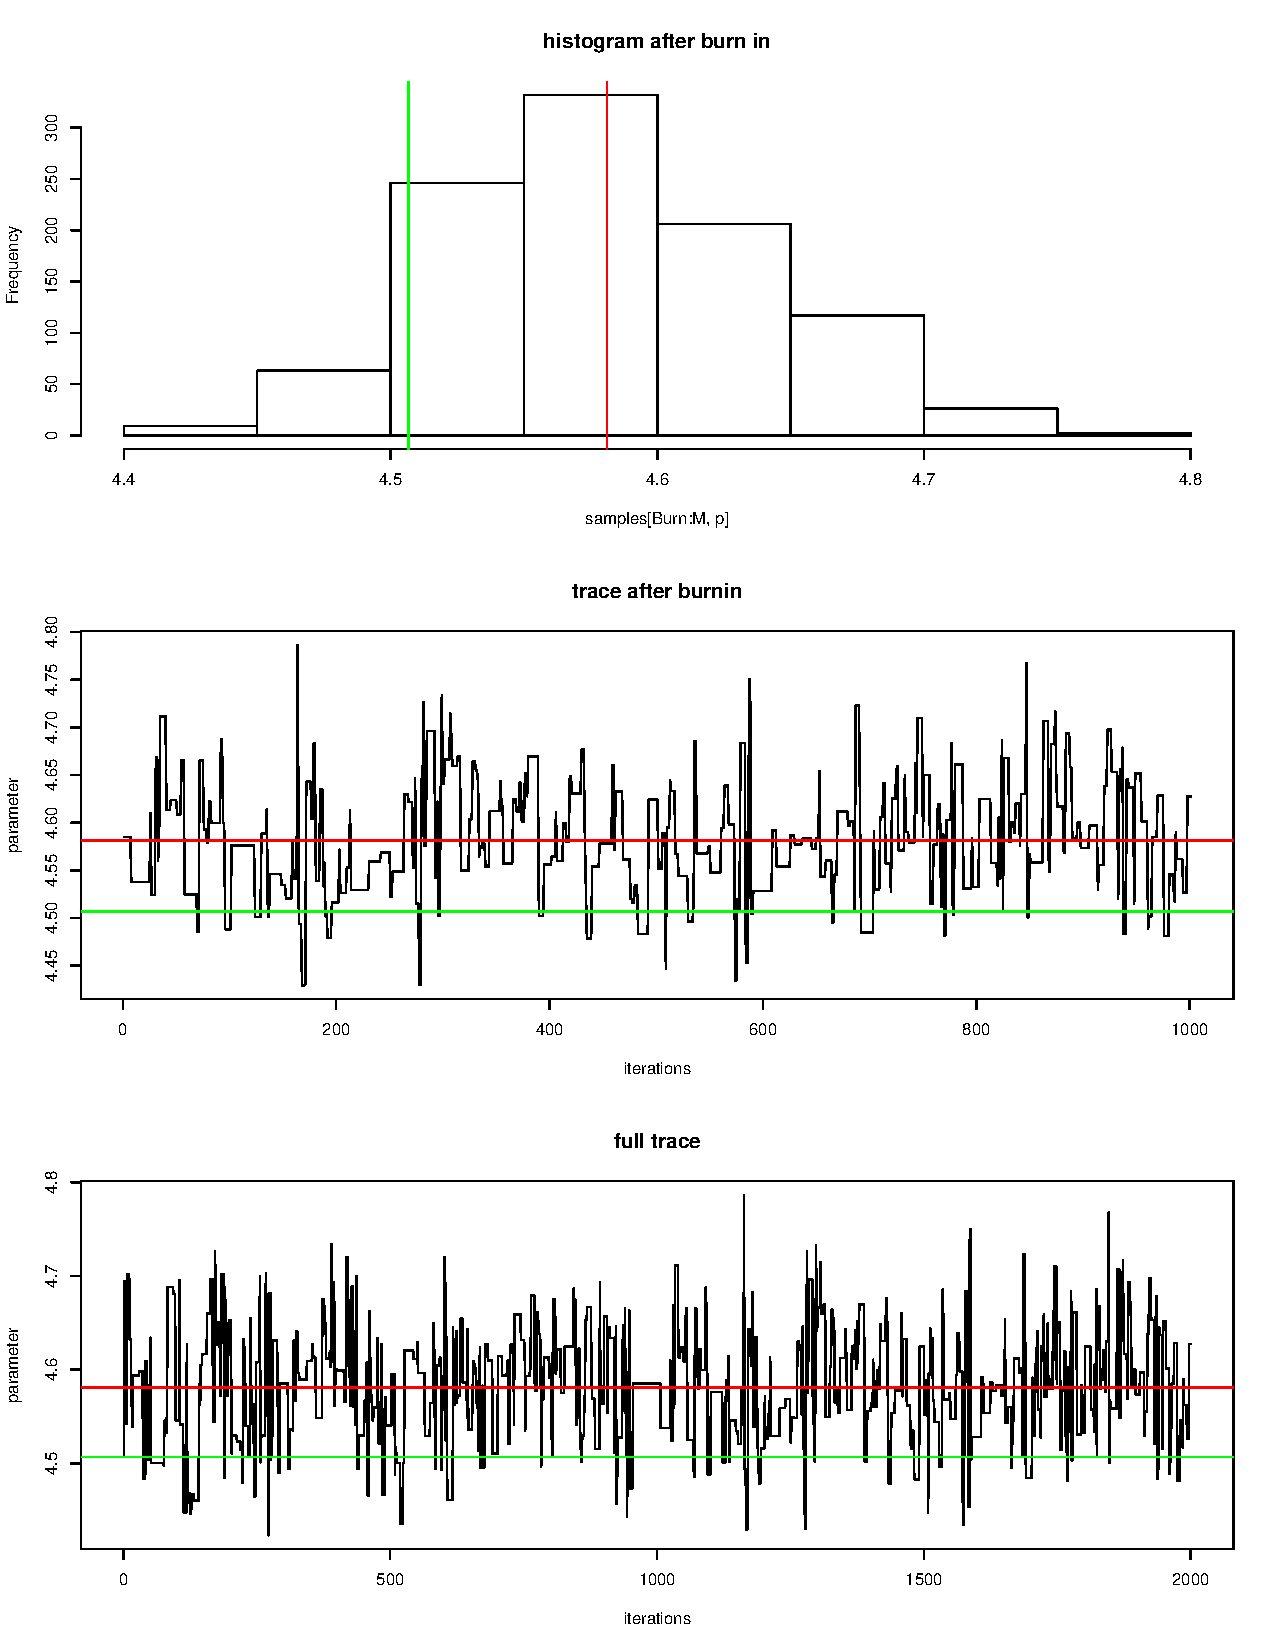
\includegraphics[scale=0.4]{16}
\clearpage
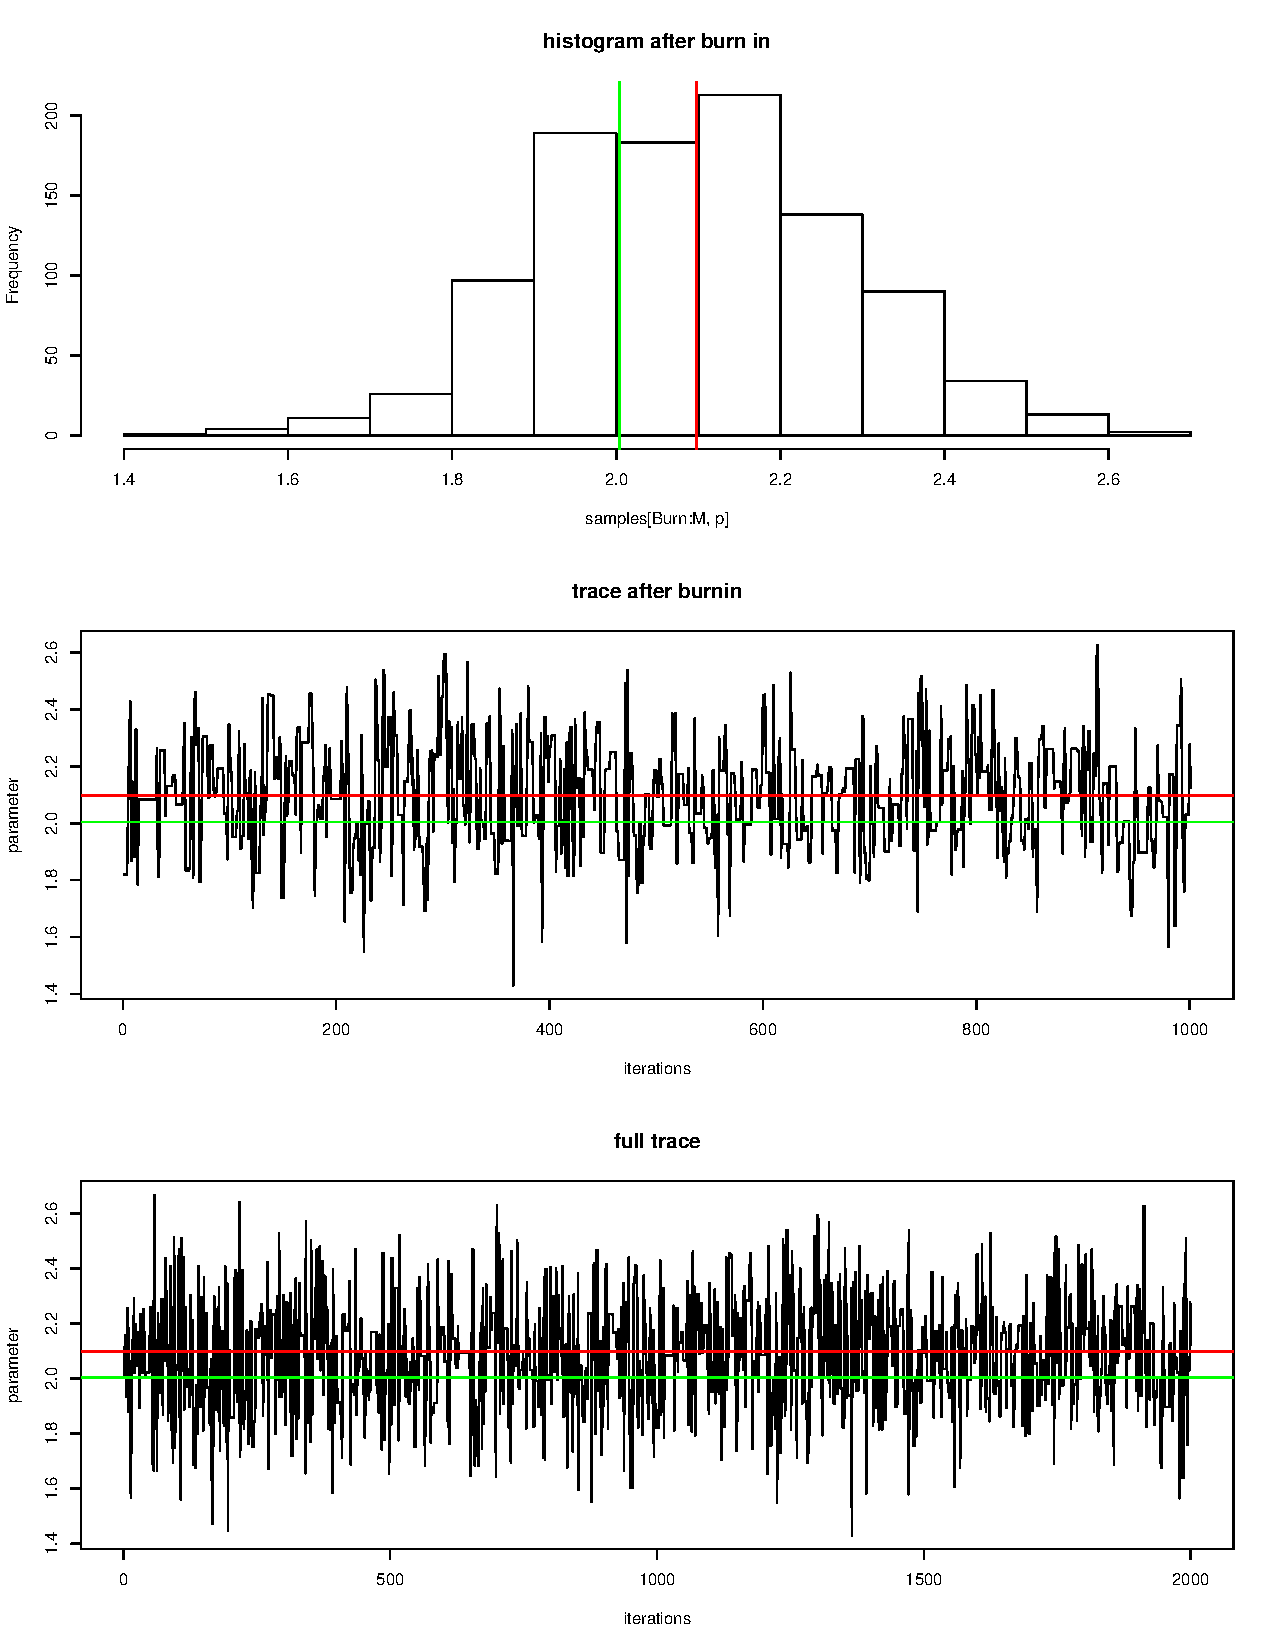
\includegraphics[scale=0.4]{17}  % scales figure to 35%\\
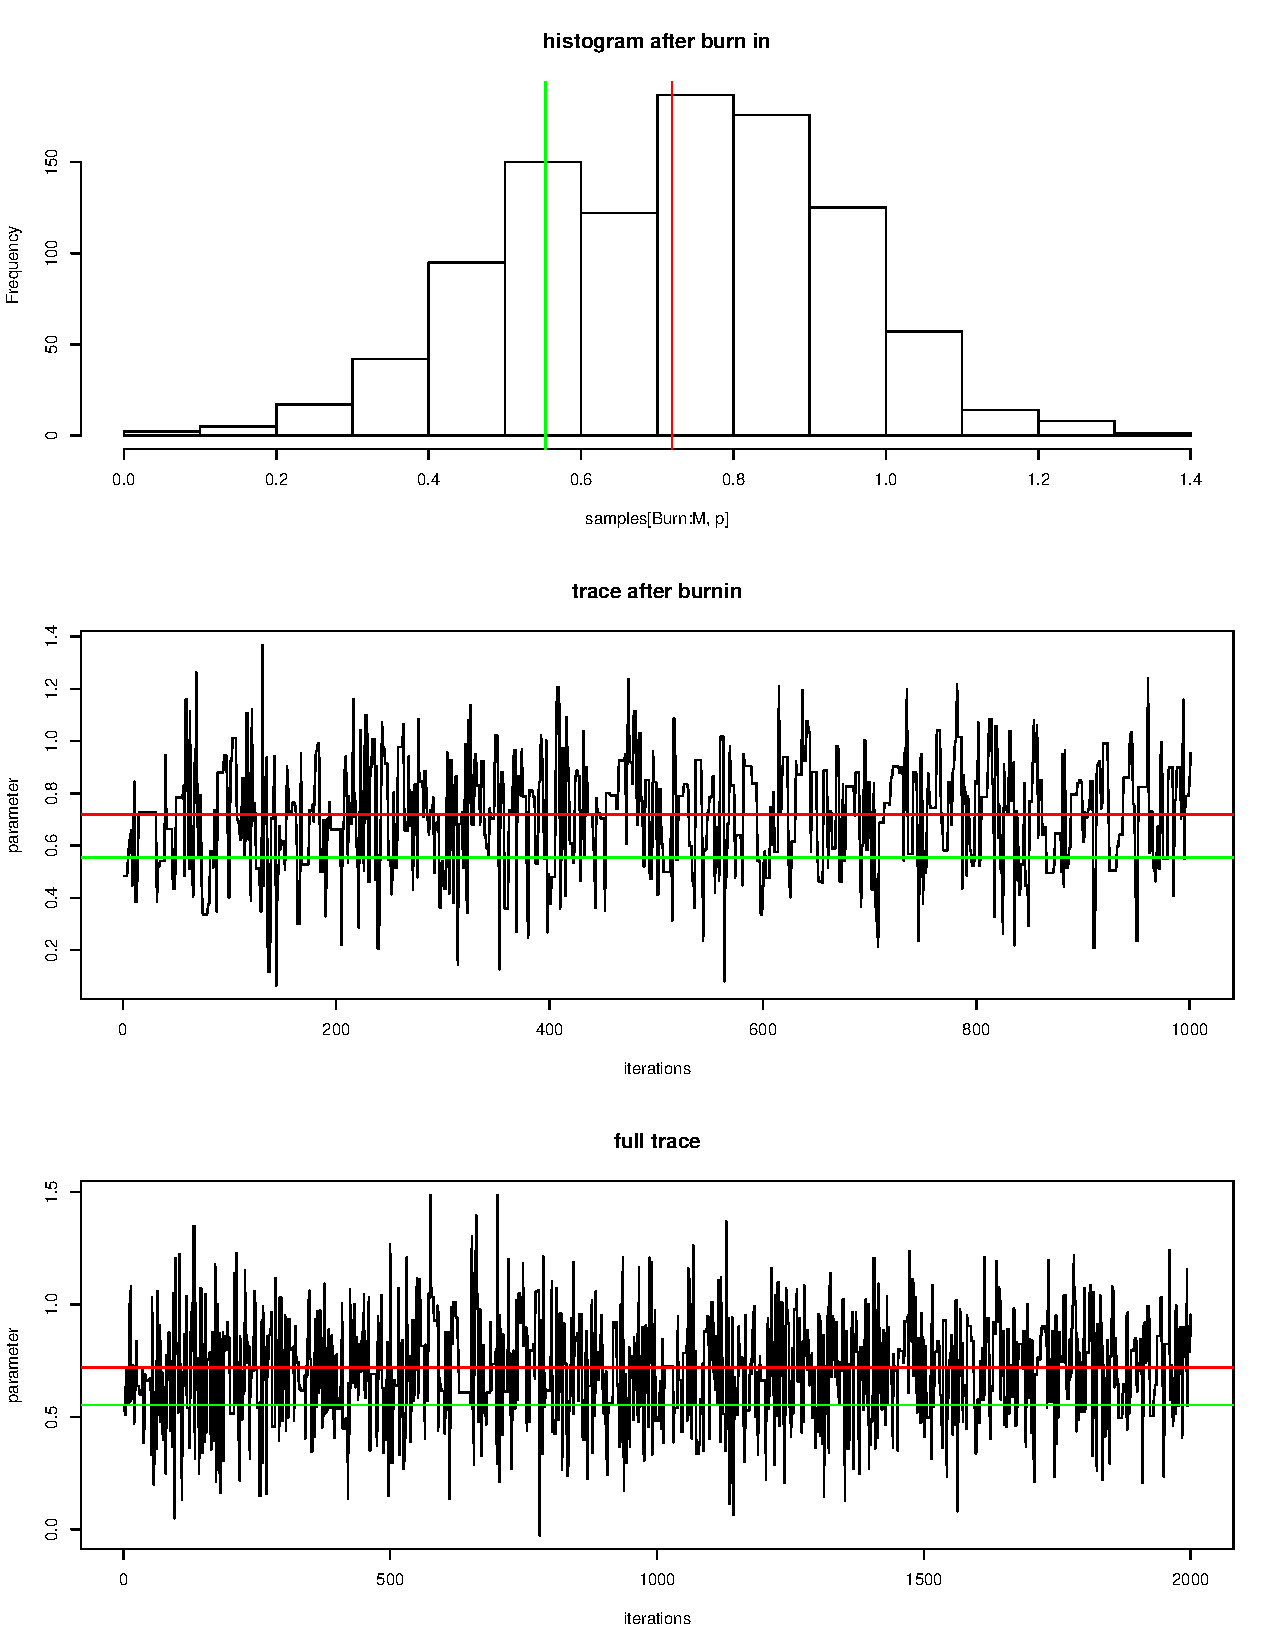
\includegraphics[scale=0.4]{18}
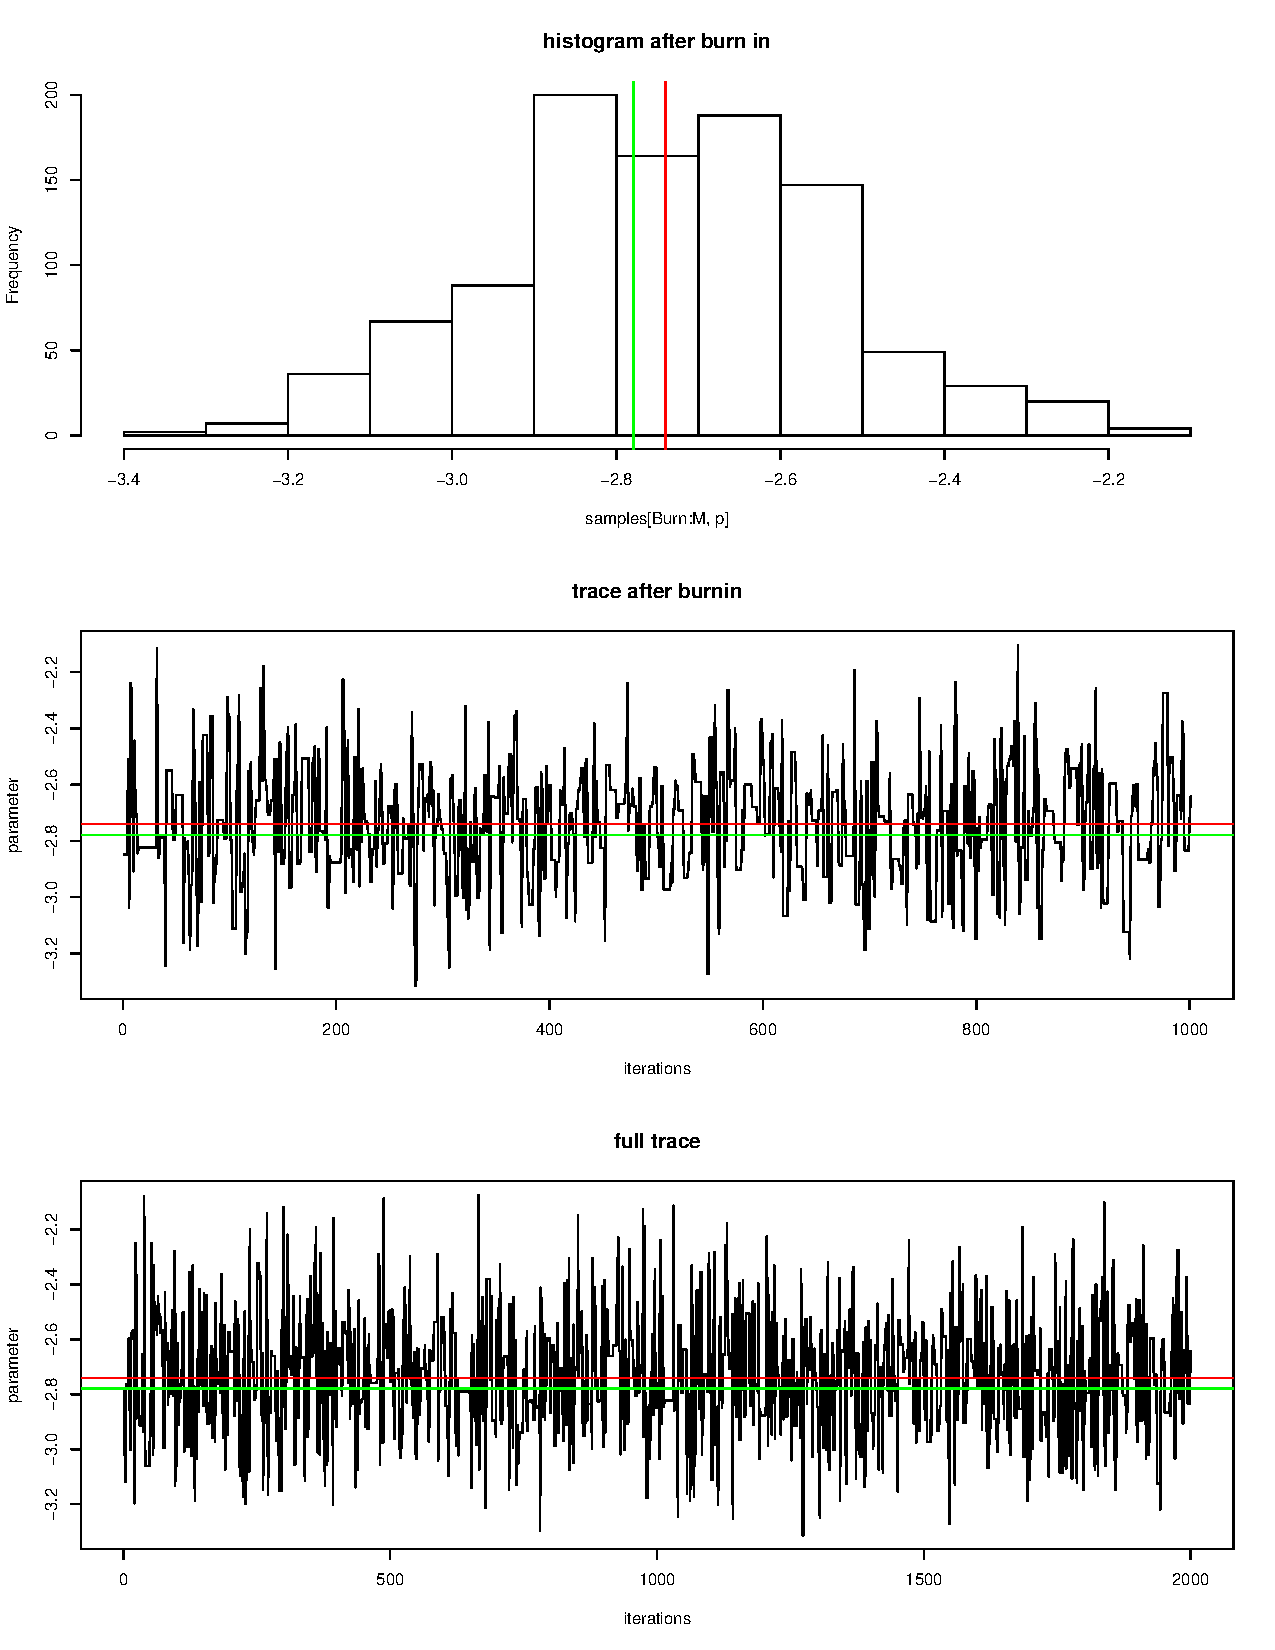
\includegraphics[scale=0.4]{19}
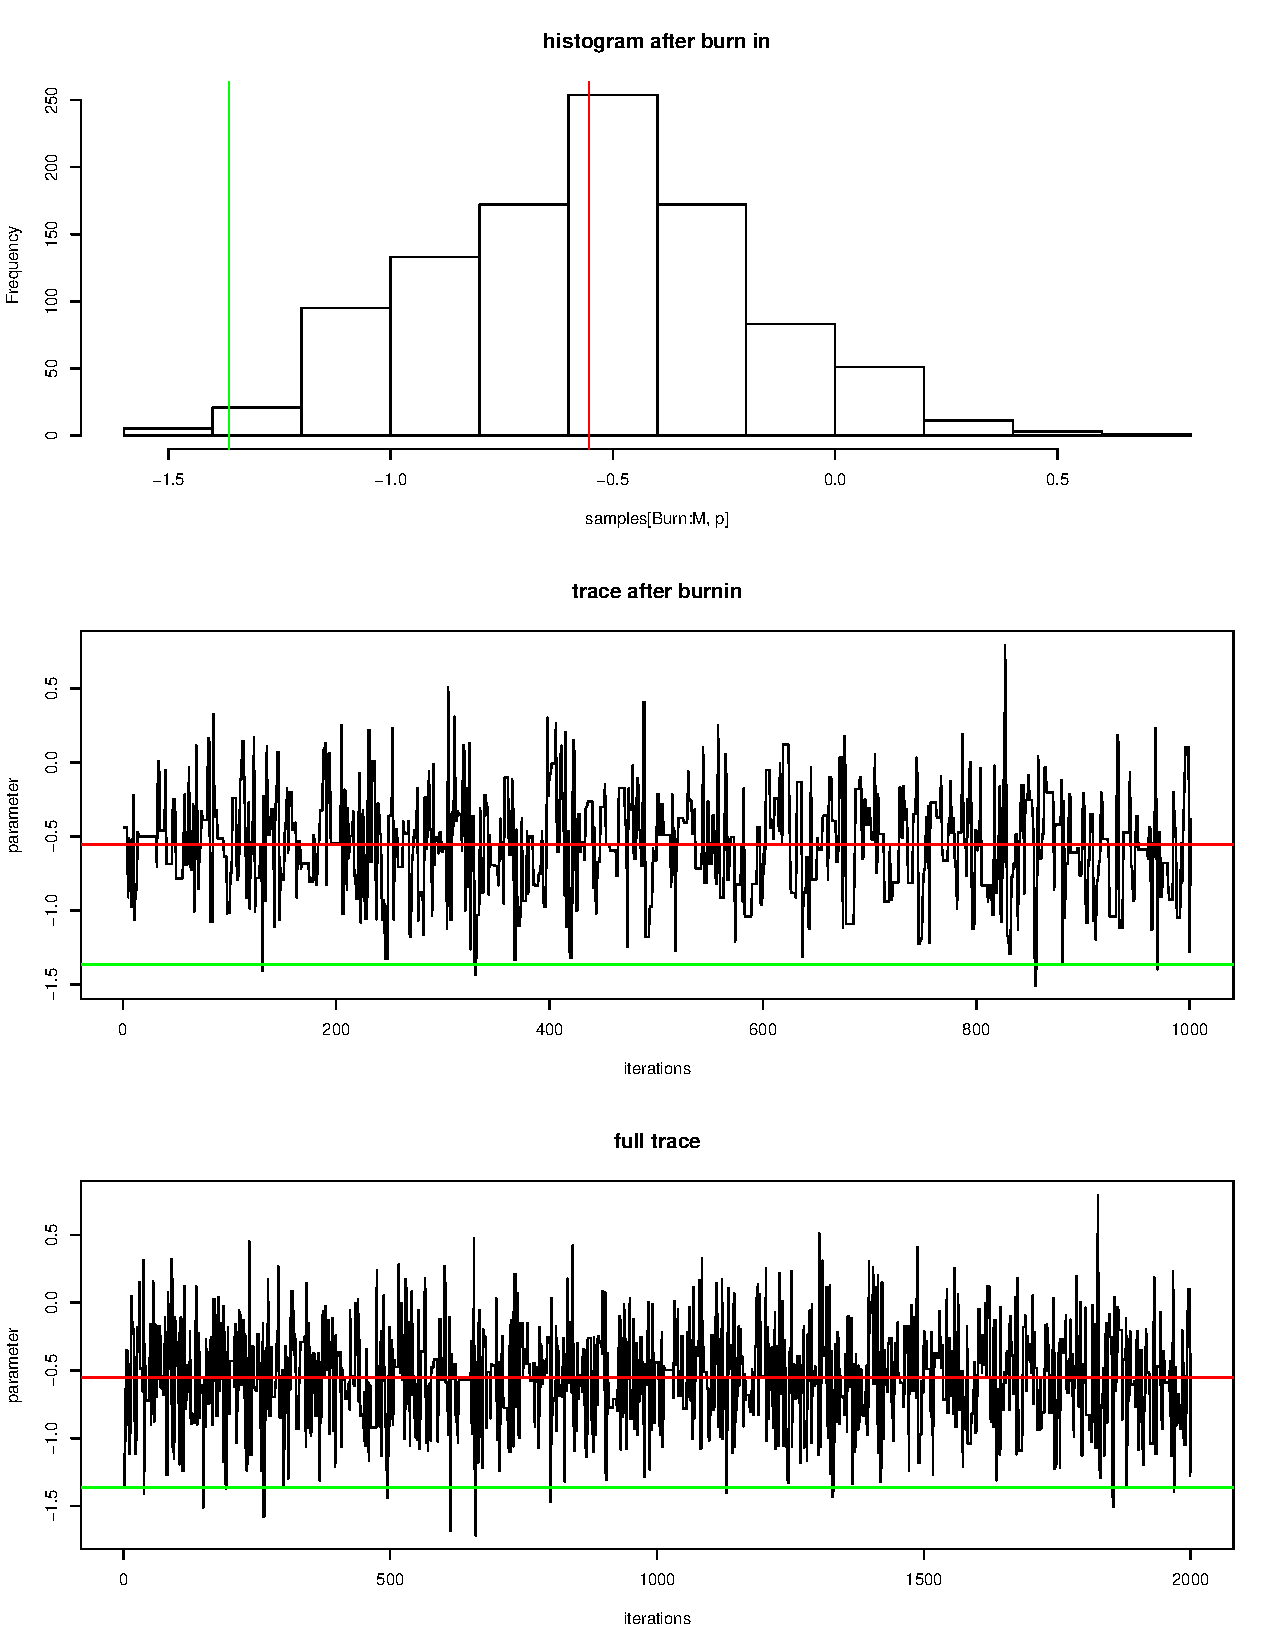
\includegraphics[scale=0.4]{20}
%
%
%
%
%
\clearpage
\section{PGAS Implementation}
\subsection{Over time T}
\subsubsection{The Model:}
\begin{itemize}
\item[] \underline{parameter vector:} for $d=1,\ldots,D$
\begin{align*}
\bs{\theta_d}=(\phi_d,\bs{\beta_{Z,d}},\bs{\beta_{W,d}},u_d)
\end{align*}
\item[] \underline{state equations:} for $d=1,\ldots,D$
\begin{align*}
%\log(\alpha_{t,d}) &= \phi_d\log(\alpha_{t-1,d}) +  \bs{z_{t}}^{\top} \bs{\beta_{Z,d}} +\bs{w}^{\top}\bs{v_{t}}\bs{\beta_{W,d}} + u_d + \epsilon_t\;, \epsilon_t \sim N(0,\sigma_{\epsilon}^2)\\
%\Rightarrow& p\left(\log(\alpha_{t,d})\given \log(\alpha_{t-1,d}),\bs{\theta_d}\right)=
%
%
%
x_{t,d}&= \phi_d x_{t-1,d} +  \bs{z_{t}}^{\top} \bs{\beta_{Z,d}} +\bs{w}^{\top}\bs{V_{t}}\bs{\beta_{W,d}} + u_d + \epsilon_t\;, \epsilon_t \sim N(0,\sigma_{\epsilon}^2)\\
p(x_{t,d}\given x_{t-1,d},\bs{\theta_d})&=N(x_{t,d}\given \mu_{x_{d}}, \sigma_{x_{d}}^2)\\
\mu_{x_{d}}&=\phi_d x_{t-1,d} +  \bs{z_{t}}^{\top} \bs{\beta_{Z,d}} +\bs{w}^{\top}\bs{V_{t}}\bs{\beta_{W,d}} + u_d\\ \sigma_{x_{d}}^2&=\sigma_{\epsilon}^2\\
\Rightarrow \bs{x_{t}}&=\left(x_{t,1},\ldots,x_{t,D}\right)
\end{align*}
\item[] \underline{measurement equations}
\begin{align*}
\bs{y_t}&= B\left(\exp(\bs{x_t})\right)^{-1}\times\prodd (y_{t,d})^{\exp((x_{t,d}-1)}\\
p(\bs{y_t}\given \bs{x_{t}}) &= \Dir\left(\bs{y_t}\given  \exp(\bs{x_t})\right)
%\underset{n,t}{\overset{ind.}{\sim}} 
\end{align*}
\end{itemize}
\clearpage
\underline{In Detail:}
\clearpage
\subsubsection{PGAS:}
\begin{itemize}
\item[$s=0$] Initialization: Set $\rt(0)$ and $X_{\seqtT}^{\mathcal{R}}(0)$ arbitrarily or by sampling from a SMC-AS pre-run targeting $p_{}(x_{\seqtT}\given y_{\seqtT},\rt(0))$ i.e. $X_{\seqtT}^{\mathcal{R}}(0)\sim \widehat{p}_{}(x_{\seqtT}\given y_{\seqtT},\rt(0))$.
\item[$s\geq 1$] Sample between $p
(\rt\given x_{\seqtT},y_{\seqtT})$ and a SMC-AS  
approx. to $p(x_{\seqtT}\given y_{\seqtT},\rt)$:
\begin{itemize}
\item[I.] Sample $\rt(s)\sim p
(\cdot\given X_{\seqtT}^{\mathcal{R}}(s-1),y_{\seqtT})$\;.
\item[II.] Run a SMC-AS targeting
$p_{}(x_{\seqtT}\given y_{\seqtT},\rt(s))$ conditional \\on $X_{\seqtT}^{\mathcal{R}}(s-1)$ following the  \textsc{Algorithm} below\;.
\item[III.] Sample $X_{\seqtT}^{\mathcal{R}}(s)\sim\widehat{p}_{}(\cdot\given y_{\seqtT},\rt(s))$\;.
\end{itemize}
\end{itemize}
\clearpage
\underline{In Detail:}
\clearpage
\subsubsection{Conditional SMC/BPF with AS:}
\textbf{\texttt{Algorithm}:}\label{ag:2}
\begin{itemize}
\item[\texttt{START}]
\begin{itemize}
\item[] \underline{\textit{For $t=1$:}}
\item[1.] For $i=1,\ldots,M-1$: \\ Sample $X_{1}^i\sim q_1(\cdot)$ 
\item[\tc{PineGreen}{2.}] \tc{PineGreen}{Conditioning: For $i=M$:\\ Set $X_{1}^M=X_{1}^\mathcal{R}$}
\item[3.]  For $i=1,\ldots,M$: \\Compute unnormalized  $w_{1}(X_{1}^i)$ and normalized weights  $W_{1}^i$.
\item[] \underline{\textit{For $t=2$ to $T$:}}
\item[] For $i=1,\ldots,M-1$:
\item[4.] Sample $A_{t}^i\sim \mathcal{M}(\cdot\given \bs{W}_{t-1})$
\item[5.] Sample $X_{t}^i\sim q_t(\cdot\given X_{t-1}^{A_{t}^i})$ for $i=1,\ldots,M-1$
\item[] For $i=M$:
\item[\tc{PineGreen}{6.}] \tc{PineGreen}{Conditioning: Set $X_{t}^M=X_{t}^\mathcal{R}$}
\item[] For $i=1,\ldots,M$:
\item[\tc{purple}{7.}] \tc{purple}{AS: Compute $\asW$ and sample $A_{t}^M\sim \mathcal{M}(1,\bs{p}=\asWb)$}
\item[8.] Set $X_{\seqt}^i\leftarrow\big(X^{A_{t}^i}_{\seqtm},X_{t}^i)$ for $i=1,\ldots,M$
\item[9.] Compute unnormalized  $w_{t}(X_{t}^i)$ and normalized weights  $W_{t}^i$
%\item[\tc{blue}{10.}] \tc{blue}{Return a particle trajectory by sampling $X_\seqnN\sim p()$}
\end{itemize}
\item[\texttt{END}]
\end{itemize}
Above \texttt{Algorithm} allows to obtain a sample $X_{\seqtT}^*$ from the SMC-AS approximation to $p_{\rt}(x_\seqnN\given y_{\seqtT})$. To this end, draw an index $k$ with probability $P(k=i)=W_{T}^{i}$ i.e. $k\sim \mathcal{M}(1,\bs{p}=\bs{W_{T}})$ and set $X_{\seqtT}^*=X_{\seqtT}^{k}$ where $\left\{W_{T}^i,X_{\seqtT}^i\right\}_{i=1}^M$ is  obtained from step 8.-9. at iteration $t=T$. To shorten notation, denote this step by $X_{\seqtT}^* \sim \widehat{p}_{\rt}(x_{\seqtT}\given y_{\seqtT})$.
\clearpage
\underline{In Detail:}
\clearpage
\subsection{Over cross section N and time T}
\subsubsection{The Model:}
\clearpage
\underline{In Detail:}
\clearpage
\subsubsection{PGAS:}
\begin{itemize}
\item[$s=0$] Initialization: Set $\rt(0)$ and $X_{\seqnN,\seqtT}^{\mathcal{R}}(0)$ arbitrarily (or by sampling from a SMC-AS pre-run targeting $p_{\rt(0)}(x_{\seqnN,\seqtT}\given y_{\seqnN,\seqtT})$ i.e. $X_{\seqnN,\seqtT}^{\mathcal{R}}(0)\sim \widehat{p}_{\rt(0)}(x_{\seqnN,\seqtT}\given y_{\seqnN,\seqtT})$).
\item[$s\geq 1$] Sample between $p
(\rt\given x_{\seqnN,\seqtT},y_{\seqnN,\seqtT})$ and a SMC-AS  
approx. to $\p(x_{\seqnN,\seqtT}\given y_{\seqnN,\seqtT})$:
\begin{itemize}
\item[I.] Sample $\rt(s)\sim p
(\cdot\given X_{\seqnN,\seqtT}^{\mathcal{R}}(s-1),y_{\seqnN,\seqtT})$\;.
\item[II.] Run a SMC-AS targeting
$p_{\rt(s)}(x_{\seqnN,\seqtT}\given y_{\seqnN,\seqtT})$ conditional \\on $X_{\seqnN,\seqtT}^{\mathcal{R}}(s-1)$ following the  \textsc{Algorithm} below\;.
\item[III.] Sample $X_{\seqnN,\seqtT}^{\mathcal{R}}(s)\sim\widehat{p}_{\rt(s)}(\cdot\given y_{\seqnN,\seqtT})$\;.
\end{itemize}
\end{itemize}
\clearpage
\underline{In Detail:}
\clearpage
\subsubsection{Conditional SMC/BPF with AS:}
\textbf{\texttt{Algorithm}:}\label{ag:2}
\begin{itemize}
\item[\texttt{START}]
\item[] \underline{\textit{For $n=1,\ldots,N$:}}
\begin{itemize}
\item[] \underline{\textit{For $t=1$:}}
\item[1.] For $i=1,\ldots,M-1$: \\ Sample $X_{n,1}^i\sim q_1(\cdot)$ 
\item[\tc{PineGreen}{2.}] \tc{PineGreen}{Conditioning: For $i=M$:\\ Set $X_{n,1}^M=X_{n,1}^\mathcal{R}$}
\item[3.]  For $i=1,\ldots,M$: \\Compute unnormalized  $w_{n,1}(X_{n,1}^i)$ and normalized weights  $W_{n,1}^i$.
\item[] \underline{\textit{For $t=2$ to $T$:}}
\item[] For $i=1,\ldots,M-1$:
\item[4.] Sample $A_{n,t}^i\sim \mathcal{M}(\cdot\given \bs{W}_{n,t-1})$
\item[5.] Sample $X_{n,t}^i\sim q_t(\cdot\given X_{n,t-1}^{A_{n,t}^i})$ for $i=1,\ldots,M-1$
\item[] For $i=M$:
\item[\tc{PineGreen}{6.}] \tc{PineGreen}{Conditioning: Set $X_{n,t}^M=X_{n,t}^\mathcal{R}$}
\item[] For $i=1,\ldots,M$:
\item[\tc{purple}{7.}] \tc{purple}{AS: Compute $\asW$ and sample $A_{n,t}^M\sim \mathcal{M}(1,\bs{p}=\asWb)$}
\item[8.] Set $X_{n,\seqt}^i\leftarrow\big(X^{A_{n,t}^i}_{n,\seqtm},X_{n,t}^i)$ for $i=1,\ldots,M$
\item[9.] Compute unnormalized  $w_{n,t}(X_{n,t}^i)$ and normalized weights  $W_{n,t}^i$
%\item[\tc{blue}{10.}] \tc{blue}{Return a particle trajectory by sampling $X_\seqnN\sim p()$}
\end{itemize}
\item[\texttt{END}]
\end{itemize}
Above \texttt{Algorithm} allows to obtain a sample $X_{\seqnN,\seqtT}^*$ from the SMC-AS approximation to $p_{\rt}(x_\seqnN\given y_{\seqnN,\seqtT})$. To this end, draw an index $k$ with probability $P(k=i)=W_{N,T}^{i}$ i.e. $k\sim \mathcal{M}(1,\bs{p}=\bs{W_{N,T}})$ and set $X_{\seqnN,\seqtT}^*=X_{\seqnN,\seqtT}^{k}$ where $\left\{W_{N,T}^i,X_{\seqnN,\seqtT}^i\right\}_{i=1}^M$ is  obtained from step 8.-9. at iteration $n=N$,$t=T$. To shorten notation, denote this step by $X_{\seqnN,\seqtT}^* \sim \widehat{p}_{\rt}(x_{\seqnN,\seqtT}\given y_{\seqnN,\seqtT})$.
\clearpage
\underline{In Detail:}
%
%
%
%
%
%_________________ End of Main Matter_________________%

\clearpage

%_________________ Reference Section _______________%

\phantomsection                                   % allows for correct link to Table of Contents
\addcontentsline{toc}{section}{References}        % Adds the line "References" to Table of contents
\onehalfspacing


%\printbibliography % print the bibliography using BibLaTex


%% alternative using BibTeX
%\bibliographystyle{econometrica}                  % sets the style for the Bibliography
%\bibliography{mybibfile}                         % Uses the Bibtex-file mybibfile.bib


\clearpage
%_________________ Space for Supplementary Material _______________%
\appendix
\numberwithin{equation}{section} %restarts equation numbering with 1 and adds the appendix in front
\numberwithin{table}{section} %same for Tables
\numberwithin{figure}{section} %and for Figures

%\section{Appendix 1}
%
%Some Information relegated to the appendix.
%\begin{equation}
%    MV=PQ
%\end{equation}
%
%\pagebreak
%
%\section{Supplementary Tables}
%



%\begin{table}[h!] % h! places the float at this place, use t for top or b for bottom
%\caption{Title of the table}
%\label{tab:SuppTable1}
%\centering
% \begin{tabular}{lcr}
%   Another & small & table\\
%\toprule
%   left aligned & centered & right aligned \\
%   \multicolumn{2}{c}{Text over two columns} & third column \\
%\bottomrule
%\end{tabular}
%\caption*{\footnotesize{\emph{Notes:} Add the description here}}
%\end{table}

\clearpage


\end{document}
